\documentclass[twoside]{book}

% Packages required by doxygen
\usepackage{fixltx2e}
\usepackage{calc}
\usepackage{doxygen}
\usepackage[export]{adjustbox} % also loads graphicx
\usepackage{graphicx}
\usepackage[utf8]{inputenc}
\usepackage{makeidx}
\usepackage{multicol}
\usepackage{multirow}
\PassOptionsToPackage{warn}{textcomp}
\usepackage{textcomp}
\usepackage[nointegrals]{wasysym}
\usepackage[table]{xcolor}

% Font selection
\usepackage[T1]{fontenc}
\usepackage[scaled=.90]{helvet}
\usepackage{courier}
\usepackage{amssymb}
\usepackage{sectsty}
\renewcommand{\familydefault}{\sfdefault}
\allsectionsfont{%
  \fontseries{bc}\selectfont%
  \color{darkgray}%
}
\renewcommand{\DoxyLabelFont}{%
  \fontseries{bc}\selectfont%
  \color{darkgray}%
}
\newcommand{\+}{\discretionary{\mbox{\scriptsize$\hookleftarrow$}}{}{}}

% Page & text layout
\usepackage{geometry}
\geometry{%
  a4paper,%
  top=2.5cm,%
  bottom=2.5cm,%
  left=2.5cm,%
  right=2.5cm%
}
\tolerance=750
\hfuzz=15pt
\hbadness=750
\setlength{\emergencystretch}{15pt}
\setlength{\parindent}{0cm}
\setlength{\parskip}{0.2cm}
\makeatletter
\renewcommand{\paragraph}{%
  \@startsection{paragraph}{4}{0ex}{-1.0ex}{1.0ex}{%
    \normalfont\normalsize\bfseries\SS@parafont%
  }%
}
\renewcommand{\subparagraph}{%
  \@startsection{subparagraph}{5}{0ex}{-1.0ex}{1.0ex}{%
    \normalfont\normalsize\bfseries\SS@subparafont%
  }%
}
\makeatother

% Headers & footers
\usepackage{fancyhdr}
\pagestyle{fancyplain}
\fancyhead[LE]{\fancyplain{}{\bfseries\thepage}}
\fancyhead[CE]{\fancyplain{}{}}
\fancyhead[RE]{\fancyplain{}{\bfseries\leftmark}}
\fancyhead[LO]{\fancyplain{}{\bfseries\rightmark}}
\fancyhead[CO]{\fancyplain{}{}}
\fancyhead[RO]{\fancyplain{}{\bfseries\thepage}}
\fancyfoot[LE]{\fancyplain{}{}}
\fancyfoot[CE]{\fancyplain{}{}}
\fancyfoot[RE]{\fancyplain{}{\bfseries\scriptsize Generated on Wed Apr 29 2015 15\+:36\+:15 for C\+U\+D\+A\+D\+Clusterer by Doxygen }}
\fancyfoot[LO]{\fancyplain{}{\bfseries\scriptsize Generated on Wed Apr 29 2015 15\+:36\+:15 for C\+U\+D\+A\+D\+Clusterer by Doxygen }}
\fancyfoot[CO]{\fancyplain{}{}}
\fancyfoot[RO]{\fancyplain{}{}}
\renewcommand{\footrulewidth}{0.4pt}
\renewcommand{\chaptermark}[1]{%
  \markboth{#1}{}%
}
\renewcommand{\sectionmark}[1]{%
  \markright{\thesection\ #1}%
}

% Indices & bibliography
\usepackage{natbib}
\usepackage[titles]{tocloft}
\setcounter{tocdepth}{3}
\setcounter{secnumdepth}{5}
\makeindex

% Hyperlinks (required, but should be loaded last)
\usepackage{ifpdf}
\ifpdf
  \usepackage[pdftex,pagebackref=true]{hyperref}
\else
  \usepackage[ps2pdf,pagebackref=true]{hyperref}
\fi
\hypersetup{%
  colorlinks=true,%
  linkcolor=blue,%
  citecolor=blue,%
  unicode%
}

% Custom commands
\newcommand{\clearemptydoublepage}{%
  \newpage{\pagestyle{empty}\cleardoublepage}%
}


%===== C O N T E N T S =====

\begin{document}

% Titlepage & ToC
\hypersetup{pageanchor=false,
             bookmarks=true,
             bookmarksnumbered=true,
             pdfencoding=unicode
            }
\pagenumbering{roman}
\begin{titlepage}
\vspace*{7cm}
\begin{center}%
{\Large C\+U\+D\+A\+D\+Clusterer \\[1ex]\large 0.\+1 }\\
\vspace*{1cm}
{\large Generated by Doxygen 1.8.9.1}\\
\vspace*{0.5cm}
{\small Wed Apr 29 2015 15:36:15}\\
\end{center}
\end{titlepage}
\clearemptydoublepage
\tableofcontents
\clearemptydoublepage
\pagenumbering{arabic}
\hypersetup{pageanchor=true}

%--- Begin generated contents ---
\chapter{Main Page}
\label{index}\hypertarget{index}{}A fast implementation of the density cluster algorithm in C\+U\+D\+A of biological datasets.

C\+U\+D\+A\+D\+Clusterer uses the .xtc Groomacs file extension.

\subsection*{Requirements }


\begin{DoxyItemize}
\item C\+Make 3.\+2.\+1
\item G\+C\+C 4.\+9.\+2
\item C\+U\+D\+A 7.\+0
\item Boost 1.\+57
\end{DoxyItemize}

{\bfseries O\+B\+S\+:} These requirements were tested and proved to work. Feel free to test older versions of the requirements

\subsection*{T\+O\+D\+O }


\begin{DoxyItemize}
\item \mbox{[}x\mbox{]} .xtc file parser \mbox{[}I\+M\+P\mbox{]}
\item \mbox{[} \mbox{]} C\+U\+D\+A clusterer kernel
\item \mbox{[} \mbox{]} Dimentionality reduction
\item \mbox{[} \mbox{]} Data Visualizer
\end{DoxyItemize}

labels\+:
\begin{DoxyItemize}
\item \mbox{[}D\+O\+N\mbox{]} -\/ Done
\item \mbox{[}I\+M\+P\mbox{]} -\/ To be improoved
\item \mbox{[}B\+U\+G\mbox{]} -\/ Buggy and experimental
\end{DoxyItemize}

\subsection*{Credits }

{\bfseries Author\+:} \href{https://github.com/tlgimenes}{\tt Tiago L\+O\+B\+A\+T\+O G\+I\+M\+E\+N\+E\+S}\+: $\ast$tlgimenes.com$\ast$

{\bfseries Contributors\+:} Maybe you ! 
\chapter{Hierarchical Index}
\section{Class Hierarchy}
This inheritance list is sorted roughly, but not completely, alphabetically\+:\begin{DoxyCompactList}
\item \contentsline{section}{adjacency\+\_\+graph}{\pageref{classadjacency__graph}}{}
\item \contentsline{section}{cluster\+:\+:dbscan}{\pageref{classcluster_1_1dbscan}}{}
\begin{DoxyCompactList}
\item \contentsline{section}{cluster\+:\+:cpu\+:\+:dbscan}{\pageref{classcluster_1_1cpu_1_1dbscan}}{}
\end{DoxyCompactList}
\item \contentsline{section}{key\+\_\+value$<$ K, V $>$}{\pageref{classkey__value}}{}
\item \contentsline{section}{console\+:\+:modifier}{\pageref{classconsole_1_1modifier}}{}
\item \contentsline{section}{console\+:\+:parser}{\pageref{classconsole_1_1parser}}{}
\item \contentsline{section}{primitive$<$ T, N $>$}{\pageref{classprimitive}}{}
\item \contentsline{section}{reader\+\_\+xtc}{\pageref{classreader__xtc}}{}
\item \contentsline{section}{tree\+:\+:vp\+\_\+node\+\_\+t}{\pageref{structtree_1_1vp__node__t}}{}
\item \contentsline{section}{tree\+:\+:vp\+\_\+tree}{\pageref{classtree_1_1vp__tree}}{}
\begin{DoxyCompactList}
\item \contentsline{section}{tree\+:\+:cpu\+:\+:vp\+\_\+tree}{\pageref{classtree_1_1cpu_1_1vp__tree}}{}
\end{DoxyCompactList}
\end{DoxyCompactList}

\chapter{Class Index}
\section{Class List}
Here are the classes, structs, unions and interfaces with brief descriptions\+:\begin{DoxyCompactList}
\item\contentsline{section}{\hyperlink{classadjacency__graph}{adjacency\+\_\+graph} }{\pageref{classadjacency__graph}}{}
\item\contentsline{section}{\hyperlink{classcluster_1_1cpu_1_1dbscan}{cluster\+::cpu\+::dbscan} \\*Class for applying D\+B\+S\+C\+A\+N clustering algorithm to data }{\pageref{classcluster_1_1cpu_1_1dbscan}}{}
\item\contentsline{section}{\hyperlink{classcluster_1_1dbscan}{cluster\+::dbscan} \\*Base class for applying D\+B\+S\+C\+A\+N clustering algorithm to data }{\pageref{classcluster_1_1dbscan}}{}
\item\contentsline{section}{\hyperlink{classkey__value}{key\+\_\+value$<$ K, V $>$} \\*Key-\/\+Value class implementation }{\pageref{classkey__value}}{}
\item\contentsline{section}{\hyperlink{classconsole_1_1modifier}{console\+::modifier} }{\pageref{classconsole_1_1modifier}}{}
\item\contentsline{section}{\hyperlink{classconsole_1_1parser}{console\+::parser} \\*Class for parsing the Command Line Interface }{\pageref{classconsole_1_1parser}}{}
\item\contentsline{section}{\hyperlink{classprimitive}{primitive$<$ T, N $>$} \\*Implementation of general N-\/dimentional type }{\pageref{classprimitive}}{}
\item\contentsline{section}{\hyperlink{classreader__xtc}{reader\+\_\+xtc} \\*Class for reading trajlist and .xtc files }{\pageref{classreader__xtc}}{}
\item\contentsline{section}{\hyperlink{structtree_1_1vp__node__t}{tree\+::vp\+\_\+node\+\_\+t} \\*Vp-\/tree node for a linearized tree in an array }{\pageref{structtree_1_1vp__node__t}}{}
\item\contentsline{section}{\hyperlink{classtree_1_1vp__tree}{tree\+::vp\+\_\+tree} \\*Base class for creating vp-\/tree }{\pageref{classtree_1_1vp__tree}}{}
\item\contentsline{section}{\hyperlink{classtree_1_1cpu_1_1vp__tree}{tree\+::cpu\+::vp\+\_\+tree} \\*Base class for creating vp-\/tree }{\pageref{classtree_1_1cpu_1_1vp__tree}}{}
\end{DoxyCompactList}

\chapter{File Index}
\section{File List}
Here is a list of all documented files with brief descriptions\+:\begin{DoxyCompactList}
\item\contentsline{section}{clusterer/\hyperlink{dbscan_8hpp}{dbscan.\+hpp} \\*Definition of the class base for the dbscan clusterer }{\pageref{dbscan_8hpp}}{}
\item\contentsline{section}{clusterer/\hyperlink{dbscan__cpu_8hpp}{dbscan\+\_\+cpu.\+hpp} \\*Definition of the class specialization of dbscan for C\+P\+U }{\pageref{dbscan__cpu_8hpp}}{}
\item\contentsline{section}{knn/{\bfseries adjacency\+\_\+graph.\+hpp} }{\pageref{adjacency__graph_8hpp}}{}
\item\contentsline{section}{knn/\hyperlink{metrics_8hpp}{metrics.\+hpp} \\*Metric definitions }{\pageref{metrics_8hpp}}{}
\item\contentsline{section}{knn/\hyperlink{vp__tree_8hpp}{vp\+\_\+tree.\+hpp} \\*Vp\+\_\+tree base class implementation }{\pageref{vp__tree_8hpp}}{}
\item\contentsline{section}{knn/\hyperlink{vp__tree__cpu_8hpp}{vp\+\_\+tree\+\_\+cpu.\+hpp} \\*Vp\+\_\+tree cpu class especification }{\pageref{vp__tree__cpu_8hpp}}{}
\item\contentsline{section}{parser/\hyperlink{parser_8hpp}{parser.\+hpp} \\*C\+L\+I parser }{\pageref{parser_8hpp}}{}
\item\contentsline{section}{utils/\hyperlink{color_8hpp}{color.\+hpp} \\*Color C\+L\+I modifier }{\pageref{color_8hpp}}{}
\item\contentsline{section}{utils/\hyperlink{error_8hpp}{error.\+hpp} \\*Error repporting interface }{\pageref{error_8hpp}}{}
\item\contentsline{section}{utils/\hyperlink{reader__xtc_8hpp}{reader\+\_\+xtc.\+hpp} \\*.xtc file reader }{\pageref{reader__xtc_8hpp}}{}
\item\contentsline{section}{utils/\hyperlink{time_8hpp}{time.\+hpp} \\*Functions and tools for mesuring the execution time of a given code }{\pageref{time_8hpp}}{}
\item\contentsline{section}{utils/\hyperlink{types_8hpp}{types.\+hpp} \\*Simple type definitions }{\pageref{types_8hpp}}{}
\end{DoxyCompactList}

\chapter{Class Documentation}
\hypertarget{classadjacency__graph}{}\section{adjacency\+\_\+graph Class Reference}
\label{classadjacency__graph}\index{adjacency\+\_\+graph@{adjacency\+\_\+graph}}


The documentation for this class was generated from the following file\+:\begin{DoxyCompactItemize}
\item 
knn/adjacency\+\_\+graph.\+hpp\end{DoxyCompactItemize}

\hypertarget{classcluster_1_1cpu_1_1dbscan}{}\section{cluster\+:\+:cpu\+:\+:dbscan Class Reference}
\label{classcluster_1_1cpu_1_1dbscan}\index{cluster\+::cpu\+::dbscan@{cluster\+::cpu\+::dbscan}}


Class for applying D\+B\+S\+C\+A\+N clustering algorithm to data.  




{\ttfamily \#include $<$dbscan\+\_\+cpu.\+hpp$>$}

Inheritance diagram for cluster\+:\+:cpu\+:\+:dbscan\+:\begin{figure}[H]
\begin{center}
\leavevmode
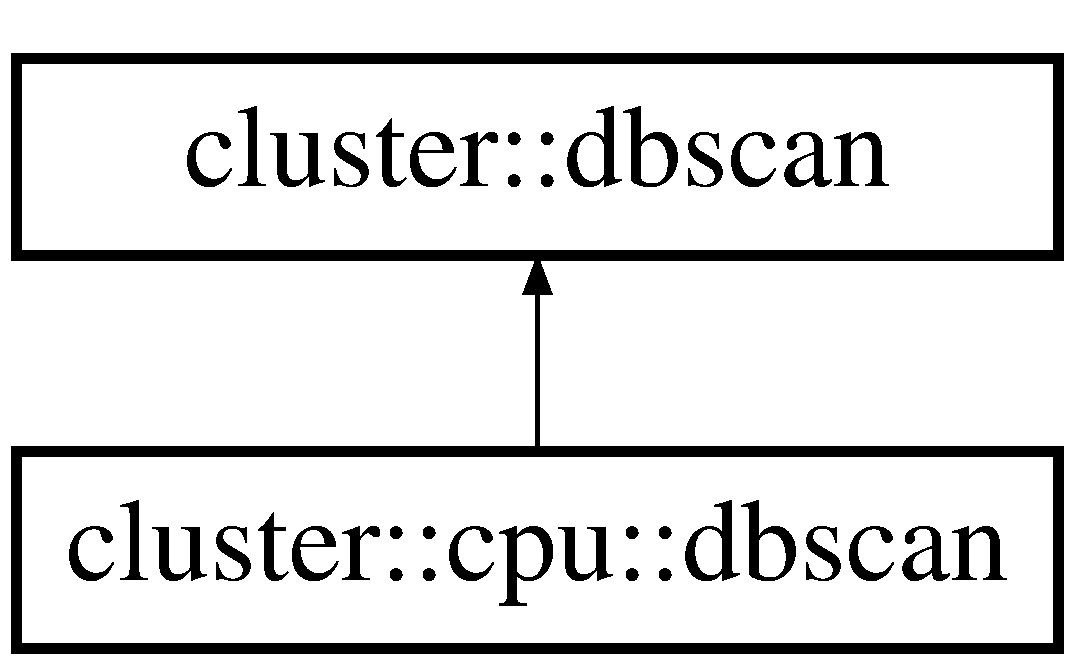
\includegraphics[height=2.000000cm]{classcluster_1_1cpu_1_1dbscan}
\end{center}
\end{figure}
\subsection*{Public Member Functions}
\begin{DoxyCompactItemize}
\item 
\hyperlink{classcluster_1_1cpu_1_1dbscan_a48d1156c8eb000f2ae8a916b31b2d492}{dbscan} (std\+::shared\+\_\+ptr$<$ const std\+::vector$<$ float $>$$>$ data, const float \hyperlink{classcluster_1_1dbscan_adffe3dee8aede13ce2068552a38e4bb9}{eps}, const int \hyperlink{classcluster_1_1dbscan_a5f424fb02ca1d736fb07f9e214a01a65}{min\+\_\+pts}, const int dim, metric\+::cpu\+::metric\+\_\+f metric=metric\+::cpu\+::euclidean)
\begin{DoxyCompactList}\small\item\em Constructor of the clusterer. \end{DoxyCompactList}\end{DoxyCompactItemize}
\subsection*{Protected Attributes}
\begin{DoxyCompactItemize}
\item 
\hypertarget{classcluster_1_1cpu_1_1dbscan_a2834cc24b1a05284d8f2d18b3d9f7ae7}{}\hyperlink{classtree_1_1cpu_1_1vp__tree}{tree\+::cpu\+::vp\+\_\+tree} \hyperlink{classcluster_1_1cpu_1_1dbscan_a2834cc24b1a05284d8f2d18b3d9f7ae7}{\+\_\+tree}\label{classcluster_1_1cpu_1_1dbscan_a2834cc24b1a05284d8f2d18b3d9f7ae7}

\begin{DoxyCompactList}\small\item\em V\+P-\/tree for the knn search. \end{DoxyCompactList}\end{DoxyCompactItemize}


\subsection{Detailed Description}
Class for applying D\+B\+S\+C\+A\+N clustering algorithm to data. 

\subsection{Constructor \& Destructor Documentation}
\hypertarget{classcluster_1_1cpu_1_1dbscan_a48d1156c8eb000f2ae8a916b31b2d492}{}\index{cluster\+::cpu\+::dbscan@{cluster\+::cpu\+::dbscan}!dbscan@{dbscan}}
\index{dbscan@{dbscan}!cluster\+::cpu\+::dbscan@{cluster\+::cpu\+::dbscan}}
\subsubsection[{dbscan}]{\setlength{\rightskip}{0pt plus 5cm}cluster\+::cpu\+::dbscan\+::dbscan (
\begin{DoxyParamCaption}
\item[{std\+::shared\+\_\+ptr$<$ const std\+::vector$<$ float $>$$>$}]{data, }
\item[{const float}]{eps, }
\item[{const int}]{min\+\_\+pts, }
\item[{const int}]{dim, }
\item[{metric\+::cpu\+::metric\+\_\+f}]{metric = {\ttfamily metric\+:\+:cpu\+:\+:euclidean}}
\end{DoxyParamCaption}
)\hspace{0.3cm}{\ttfamily [inline]}}\label{classcluster_1_1cpu_1_1dbscan_a48d1156c8eb000f2ae8a916b31b2d492}


Constructor of the clusterer. 


\begin{DoxyParams}{Parameters}
{\em data} & Data array \\
\hline
{\em eps} & Epsilon distance parameter of the D\+B\+S\+C\+A\+N algorithm \\
\hline
{\em min\+\_\+pts} & Minimal number of points for the D\+B\+S\+C\+A\+N algorithm \\
\hline
{\em dim} & Dimention of the data \\
\hline
{\em metric} & Metric function to use for the D\+B\+S\+C\+A\+N algorithm \\
\hline
\end{DoxyParams}


The documentation for this class was generated from the following file\+:\begin{DoxyCompactItemize}
\item 
clusterer/\hyperlink{dbscan__cpu_8hpp}{dbscan\+\_\+cpu.\+hpp}\end{DoxyCompactItemize}

\hypertarget{classcluster_1_1dbscan}{}\section{cluster\+:\+:dbscan Class Reference}
\label{classcluster_1_1dbscan}\index{cluster\+::dbscan@{cluster\+::dbscan}}


Base class for applying D\+B\+S\+C\+A\+N clustering algorithm to data.  




{\ttfamily \#include $<$dbscan.\+hpp$>$}

Inheritance diagram for cluster\+:\+:dbscan\+:\begin{figure}[H]
\begin{center}
\leavevmode
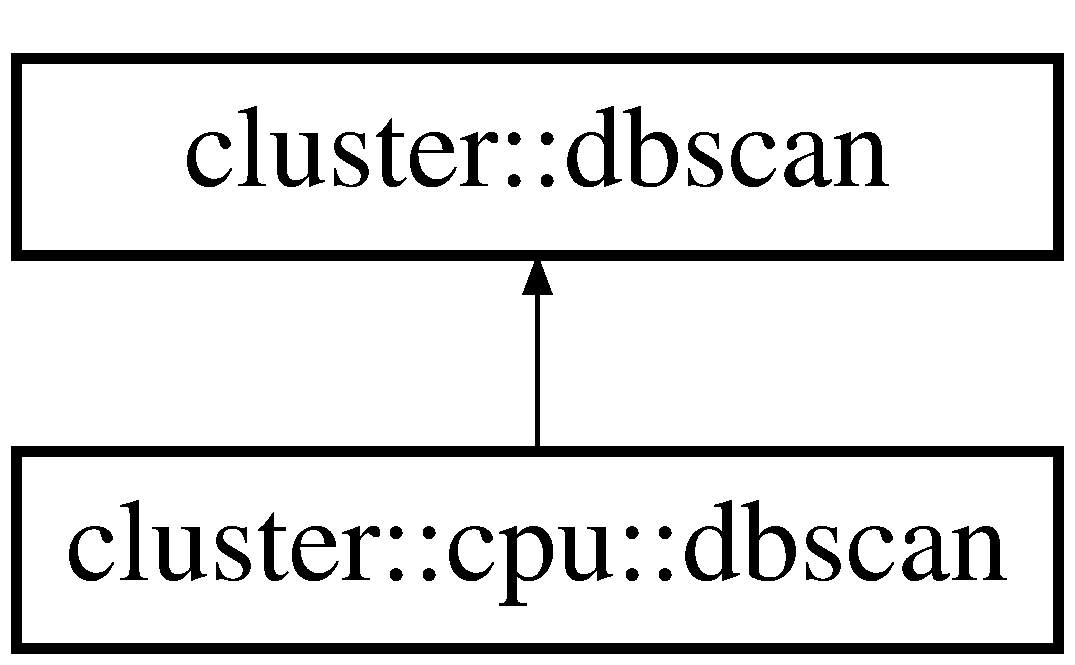
\includegraphics[height=2.000000cm]{classcluster_1_1dbscan}
\end{center}
\end{figure}
\subsection*{Public Member Functions}
\begin{DoxyCompactItemize}
\item 
\hyperlink{classcluster_1_1dbscan_af77dacb349da6976a3521297a6b50d0d}{dbscan} (std\+::shared\+\_\+ptr$<$ const std\+::vector$<$ float $>$$>$ data, const float \hyperlink{classcluster_1_1dbscan_adffe3dee8aede13ce2068552a38e4bb9}{eps}, const int \hyperlink{classcluster_1_1dbscan_a5f424fb02ca1d736fb07f9e214a01a65}{min\+\_\+pts}, const int dim)
\begin{DoxyCompactList}\small\item\em Constructor of the clusterer. \end{DoxyCompactList}\item 
\hypertarget{classcluster_1_1dbscan_adffe3dee8aede13ce2068552a38e4bb9}{}float \& \hyperlink{classcluster_1_1dbscan_adffe3dee8aede13ce2068552a38e4bb9}{eps} ()\label{classcluster_1_1dbscan_adffe3dee8aede13ce2068552a38e4bb9}

\begin{DoxyCompactList}\small\item\em Set epsilon value for the D\+B\+S\+C\+A\+N algorithm. \end{DoxyCompactList}\item 
\hypertarget{classcluster_1_1dbscan_a5f424fb02ca1d736fb07f9e214a01a65}{}int \& \hyperlink{classcluster_1_1dbscan_a5f424fb02ca1d736fb07f9e214a01a65}{min\+\_\+pts} ()\label{classcluster_1_1dbscan_a5f424fb02ca1d736fb07f9e214a01a65}

\begin{DoxyCompactList}\small\item\em Set minimun points for the D\+B\+S\+C\+A\+N algorithm. \end{DoxyCompactList}\item 
\hypertarget{classcluster_1_1dbscan_a16f0b7f5ffa65a6638df01554559ba29}{}const float \& \hyperlink{classcluster_1_1dbscan_a16f0b7f5ffa65a6638df01554559ba29}{eps} () const \label{classcluster_1_1dbscan_a16f0b7f5ffa65a6638df01554559ba29}

\begin{DoxyCompactList}\small\item\em Get epsilon value of the D\+B\+S\+C\+A\+N algorithm. \end{DoxyCompactList}\item 
\hypertarget{classcluster_1_1dbscan_a099428308e3dd233ad0098bf85fdbb7b}{}const int \& \hyperlink{classcluster_1_1dbscan_a099428308e3dd233ad0098bf85fdbb7b}{min\+\_\+pts} () const \label{classcluster_1_1dbscan_a099428308e3dd233ad0098bf85fdbb7b}

\begin{DoxyCompactList}\small\item\em Get minimun points of the D\+B\+S\+C\+A\+N algorithm. \end{DoxyCompactList}\end{DoxyCompactItemize}
\subsection*{Protected Attributes}
\begin{DoxyCompactItemize}
\item 
float \hyperlink{classcluster_1_1dbscan_a623eaf58c70c4b8af054d421addb33af}{\+\_\+eps}
\item 
int \hyperlink{classcluster_1_1dbscan_aaf6a0241678a63592356ab8e150ee511}{\+\_\+min\+\_\+pts}
\item 
int \hyperlink{classcluster_1_1dbscan_af11131046370eccd7ff4538f328106bb}{\+\_\+dim}
\item 
std\+::shared\+\_\+ptr$<$ const std\+::vector$<$ float $>$ $>$ \hyperlink{classcluster_1_1dbscan_a606f2ffd2a43d393f3d8c8a41d4280a7}{\+\_\+data}
\end{DoxyCompactItemize}


\subsection{Detailed Description}
Base class for applying D\+B\+S\+C\+A\+N clustering algorithm to data. 

\subsection{Constructor \& Destructor Documentation}
\hypertarget{classcluster_1_1dbscan_af77dacb349da6976a3521297a6b50d0d}{}\index{cluster\+::dbscan@{cluster\+::dbscan}!dbscan@{dbscan}}
\index{dbscan@{dbscan}!cluster\+::dbscan@{cluster\+::dbscan}}
\subsubsection[{dbscan}]{\setlength{\rightskip}{0pt plus 5cm}cluster\+::dbscan\+::dbscan (
\begin{DoxyParamCaption}
\item[{std\+::shared\+\_\+ptr$<$ const std\+::vector$<$ float $>$$>$}]{data, }
\item[{const float}]{eps, }
\item[{const int}]{min\+\_\+pts, }
\item[{const int}]{dim}
\end{DoxyParamCaption}
)\hspace{0.3cm}{\ttfamily [inline]}}\label{classcluster_1_1dbscan_af77dacb349da6976a3521297a6b50d0d}


Constructor of the clusterer. 


\begin{DoxyParams}{Parameters}
{\em data} & Data array \\
\hline
{\em eps} & Epsilon distance parameter of the D\+B\+S\+C\+A\+N algorithm \\
\hline
{\em min\+\_\+pts} & Minimal number of points for the D\+B\+S\+C\+A\+N algorithm \\
\hline
{\em dim} & Dimention of the data \\
\hline
\end{DoxyParams}


\subsection{Member Data Documentation}
\hypertarget{classcluster_1_1dbscan_a606f2ffd2a43d393f3d8c8a41d4280a7}{}\index{cluster\+::dbscan@{cluster\+::dbscan}!\+\_\+data@{\+\_\+data}}
\index{\+\_\+data@{\+\_\+data}!cluster\+::dbscan@{cluster\+::dbscan}}
\subsubsection[{\+\_\+data}]{\setlength{\rightskip}{0pt plus 5cm}std\+::shared\+\_\+ptr$<$const std\+::vector$<$float$>$ $>$ cluster\+::dbscan\+::\+\_\+data\hspace{0.3cm}{\ttfamily [protected]}}\label{classcluster_1_1dbscan_a606f2ffd2a43d393f3d8c8a41d4280a7}
Vector containing data \hypertarget{classcluster_1_1dbscan_af11131046370eccd7ff4538f328106bb}{}\index{cluster\+::dbscan@{cluster\+::dbscan}!\+\_\+dim@{\+\_\+dim}}
\index{\+\_\+dim@{\+\_\+dim}!cluster\+::dbscan@{cluster\+::dbscan}}
\subsubsection[{\+\_\+dim}]{\setlength{\rightskip}{0pt plus 5cm}int cluster\+::dbscan\+::\+\_\+dim\hspace{0.3cm}{\ttfamily [protected]}}\label{classcluster_1_1dbscan_af11131046370eccd7ff4538f328106bb}
Data\textquotesingle{}s dimention \hypertarget{classcluster_1_1dbscan_a623eaf58c70c4b8af054d421addb33af}{}\index{cluster\+::dbscan@{cluster\+::dbscan}!\+\_\+eps@{\+\_\+eps}}
\index{\+\_\+eps@{\+\_\+eps}!cluster\+::dbscan@{cluster\+::dbscan}}
\subsubsection[{\+\_\+eps}]{\setlength{\rightskip}{0pt plus 5cm}float cluster\+::dbscan\+::\+\_\+eps\hspace{0.3cm}{\ttfamily [protected]}}\label{classcluster_1_1dbscan_a623eaf58c70c4b8af054d421addb33af}
Epsilon parameters \hypertarget{classcluster_1_1dbscan_aaf6a0241678a63592356ab8e150ee511}{}\index{cluster\+::dbscan@{cluster\+::dbscan}!\+\_\+min\+\_\+pts@{\+\_\+min\+\_\+pts}}
\index{\+\_\+min\+\_\+pts@{\+\_\+min\+\_\+pts}!cluster\+::dbscan@{cluster\+::dbscan}}
\subsubsection[{\+\_\+min\+\_\+pts}]{\setlength{\rightskip}{0pt plus 5cm}int cluster\+::dbscan\+::\+\_\+min\+\_\+pts\hspace{0.3cm}{\ttfamily [protected]}}\label{classcluster_1_1dbscan_aaf6a0241678a63592356ab8e150ee511}
Minimal number of points Parameters 

The documentation for this class was generated from the following file\+:\begin{DoxyCompactItemize}
\item 
clusterer/\hyperlink{dbscan_8hpp}{dbscan.\+hpp}\end{DoxyCompactItemize}

\hypertarget{classkey__value}{}\section{key\+\_\+value$<$ K, V $>$ Class Template Reference}
\label{classkey__value}\index{key\+\_\+value$<$ K, V $>$@{key\+\_\+value$<$ K, V $>$}}


Key-\/\+Value class implementation.  




{\ttfamily \#include $<$types.\+hpp$>$}

\subsection*{Public Member Functions}
\begin{DoxyCompactItemize}
\item 
\hyperlink{classkey__value_ad3a7caf2cf9eff66215ee4983c2f4bce}{key\+\_\+value} (K k, V v)
\begin{DoxyCompactList}\small\item\em Constructor. \end{DoxyCompactList}\item 
\hypertarget{classkey__value_a9209ff3cf223c216f87e2da1d12a39b2}{}\hyperlink{classkey__value_a9209ff3cf223c216f87e2da1d12a39b2}{key\+\_\+value} ()\label{classkey__value_a9209ff3cf223c216f87e2da1d12a39b2}

\begin{DoxyCompactList}\small\item\em Constructs new element with default key and value. \end{DoxyCompactList}\item 
\hypertarget{classkey__value_a1dec00eb7ce57a91bd991ecc4cef02b9}{}const V \& \hyperlink{classkey__value_a1dec00eb7ce57a91bd991ecc4cef02b9}{val} () const \label{classkey__value_a1dec00eb7ce57a91bd991ecc4cef02b9}

\begin{DoxyCompactList}\small\item\em Get value. \end{DoxyCompactList}\item 
\hypertarget{classkey__value_ae07d8b9f4f22b915c31e68785fa165a5}{}const K \& \hyperlink{classkey__value_ae07d8b9f4f22b915c31e68785fa165a5}{key} () const \label{classkey__value_ae07d8b9f4f22b915c31e68785fa165a5}

\begin{DoxyCompactList}\small\item\em Get key. \end{DoxyCompactList}\item 
\hypertarget{classkey__value_aef41e9f03857a8aefcf3b6464dd8d3ce}{}V \& \hyperlink{classkey__value_aef41e9f03857a8aefcf3b6464dd8d3ce}{val} ()\label{classkey__value_aef41e9f03857a8aefcf3b6464dd8d3ce}

\begin{DoxyCompactList}\small\item\em Set value. \end{DoxyCompactList}\item 
\hypertarget{classkey__value_a5ac8d2186f8475467cba4fce559a2d17}{}K \& \hyperlink{classkey__value_a5ac8d2186f8475467cba4fce559a2d17}{key} ()\label{classkey__value_a5ac8d2186f8475467cba4fce559a2d17}

\begin{DoxyCompactList}\small\item\em Set key. \end{DoxyCompactList}\item 
\hypertarget{classkey__value_af5aed228f1e149228c34dac160463dd3}{}const \hyperlink{classkey__value}{key\+\_\+value} \& \hyperlink{classkey__value_af5aed228f1e149228c34dac160463dd3}{operator=} (const \hyperlink{classkey__value}{key\+\_\+value} \&other)\label{classkey__value_af5aed228f1e149228c34dac160463dd3}

\begin{DoxyCompactList}\small\item\em Copies key and value from one object to this. \end{DoxyCompactList}\item 
\hypertarget{classkey__value_ad272d54cc397dec6f07cfba350f7ae1d}{}bool \hyperlink{classkey__value_ad272d54cc397dec6f07cfba350f7ae1d}{operator$<$} (const \hyperlink{classkey__value}{key\+\_\+value} \&other) const \label{classkey__value_ad272d54cc397dec6f07cfba350f7ae1d}

\begin{DoxyCompactList}\small\item\em The comparision is made using the value and not the key. \end{DoxyCompactList}\end{DoxyCompactItemize}


\subsection{Detailed Description}
\subsubsection*{template$<$typename K, typename V$>$class key\+\_\+value$<$ K, V $>$}

Key-\/\+Value class implementation. 

\subsection{Constructor \& Destructor Documentation}
\hypertarget{classkey__value_ad3a7caf2cf9eff66215ee4983c2f4bce}{}\index{key\+\_\+value@{key\+\_\+value}!key\+\_\+value@{key\+\_\+value}}
\index{key\+\_\+value@{key\+\_\+value}!key\+\_\+value@{key\+\_\+value}}
\subsubsection[{key\+\_\+value}]{\setlength{\rightskip}{0pt plus 5cm}template$<$typename K , typename V $>$ {\bf key\+\_\+value}$<$ K, V $>$\+::{\bf key\+\_\+value} (
\begin{DoxyParamCaption}
\item[{K}]{k, }
\item[{V}]{v}
\end{DoxyParamCaption}
)\hspace{0.3cm}{\ttfamily [inline]}}\label{classkey__value_ad3a7caf2cf9eff66215ee4983c2f4bce}


Constructor. 


\begin{DoxyParams}{Parameters}
{\em k} & Key \\
\hline
{\em v} & Value \\
\hline
\end{DoxyParams}


The documentation for this class was generated from the following file\+:\begin{DoxyCompactItemize}
\item 
utils/\hyperlink{types_8hpp}{types.\+hpp}\end{DoxyCompactItemize}

\hypertarget{classconsole_1_1modifier}{}\section{console\+:\+:modifier Class Reference}
\label{classconsole_1_1modifier}\index{console\+::modifier@{console\+::modifier}}


{\ttfamily \#include $<$color.\+hpp$>$}

\subsection*{Public Member Functions}
\begin{DoxyCompactItemize}
\item 
\hyperlink{classconsole_1_1modifier_a0ec578bb4ac2f0bb56da5e9995fe14fe}{modifier} (enum ccode \hyperlink{classconsole_1_1modifier_ad525a786ab7b18058ca2b3e120a7ba0a}{code})
\begin{DoxyCompactList}\small\item\em color code \end{DoxyCompactList}\item 
\hypertarget{classconsole_1_1modifier_ad525a786ab7b18058ca2b3e120a7ba0a}{}enum ccode \& \hyperlink{classconsole_1_1modifier_ad525a786ab7b18058ca2b3e120a7ba0a}{code} () const \label{classconsole_1_1modifier_ad525a786ab7b18058ca2b3e120a7ba0a}

\begin{DoxyCompactList}\small\item\em Get the color code. \end{DoxyCompactList}\end{DoxyCompactItemize}
\subsection*{Friends}
\begin{DoxyCompactItemize}
\item 
\hypertarget{classconsole_1_1modifier_a1a697ad41039adb38c769e442c0238d8}{}std\+::ostream \& \hyperlink{classconsole_1_1modifier_a1a697ad41039adb38c769e442c0238d8}{operator$<$$<$} (std\+::ostream \&os, const \hyperlink{classconsole_1_1modifier}{modifier} \&mod)\label{classconsole_1_1modifier_a1a697ad41039adb38c769e442c0238d8}

\begin{DoxyCompactList}\small\item\em operator for using this class in the standard c++ output \end{DoxyCompactList}\end{DoxyCompactItemize}


\subsection{Detailed Description}
This class should be used in the following way\+: modifier red(\+F\+G\+\_\+\+R\+E\+D); std\+::cout $<$$<$ red $<$$<$ \char`\"{}this text is red\char`\"{} $<$$<$ std\+::endl; 

\subsection{Constructor \& Destructor Documentation}
\hypertarget{classconsole_1_1modifier_a0ec578bb4ac2f0bb56da5e9995fe14fe}{}\index{console\+::modifier@{console\+::modifier}!modifier@{modifier}}
\index{modifier@{modifier}!console\+::modifier@{console\+::modifier}}
\subsubsection[{modifier}]{\setlength{\rightskip}{0pt plus 5cm}console\+::modifier\+::modifier (
\begin{DoxyParamCaption}
\item[{enum ccode}]{code}
\end{DoxyParamCaption}
)\hspace{0.3cm}{\ttfamily [inline]}}\label{classconsole_1_1modifier_a0ec578bb4ac2f0bb56da5e9995fe14fe}


color code 

Constructor for the color modifier


\begin{DoxyParams}{Parameters}
{\em code} & color code for the modifier \\
\hline
\end{DoxyParams}


The documentation for this class was generated from the following file\+:\begin{DoxyCompactItemize}
\item 
utils/\hyperlink{color_8hpp}{color.\+hpp}\end{DoxyCompactItemize}

\hypertarget{classconsole_1_1parser}{}\section{console\+:\+:parser Class Reference}
\label{classconsole_1_1parser}\index{console\+::parser@{console\+::parser}}


Class for parsing the Command Line Interface.  




{\ttfamily \#include $<$parser.\+hpp$>$}

\subsection*{Static Public Member Functions}
\begin{DoxyCompactItemize}
\item 
\hypertarget{classconsole_1_1parser_ae579d789c0cc9b9b15bb7368ec54d703}{}static void \hyperlink{classconsole_1_1parser_ae579d789c0cc9b9b15bb7368ec54d703}{parse} (int argc, const char $\ast$$\ast$argv)\label{classconsole_1_1parser_ae579d789c0cc9b9b15bb7368ec54d703}

\begin{DoxyCompactList}\small\item\em Parses the command line interface. \end{DoxyCompactList}\item 
static void \hyperlink{classconsole_1_1parser_ab698f0297fcbdf6d52d32ad181c80f99}{add\+\_\+argument} (const std\+::string \&short\+\_\+form, const std\+::string \&help)
\begin{DoxyCompactList}\small\item\em Adds arguments to be parsed. \end{DoxyCompactList}\item 
static const std\+::string \hyperlink{classconsole_1_1parser_ac071bd86195d96a31cab5dad9c34aecd}{get} (const std\+::string \&arg, bool required)
\begin{DoxyCompactList}\small\item\em Gets the value of the argument. \end{DoxyCompactList}\end{DoxyCompactItemize}
\subsection*{Static Protected Member Functions}
\begin{DoxyCompactItemize}
\item 
\hypertarget{classconsole_1_1parser_a76801efa759b112e67960cbfd7fa9122}{}static void \hyperlink{classconsole_1_1parser_a76801efa759b112e67960cbfd7fa9122}{print\+\_\+help} ()\label{classconsole_1_1parser_a76801efa759b112e67960cbfd7fa9122}

\begin{DoxyCompactList}\small\item\em Prints the help in C\+L\+I. \end{DoxyCompactList}\end{DoxyCompactItemize}


\subsection{Detailed Description}
Class for parsing the Command Line Interface. 

\subsection{Member Function Documentation}
\hypertarget{classconsole_1_1parser_ab698f0297fcbdf6d52d32ad181c80f99}{}\index{console\+::parser@{console\+::parser}!add\+\_\+argument@{add\+\_\+argument}}
\index{add\+\_\+argument@{add\+\_\+argument}!console\+::parser@{console\+::parser}}
\subsubsection[{add\+\_\+argument}]{\setlength{\rightskip}{0pt plus 5cm}void console\+::parser\+::add\+\_\+argument (
\begin{DoxyParamCaption}
\item[{const std\+::string \&}]{short\+\_\+form, }
\item[{const std\+::string \&}]{help}
\end{DoxyParamCaption}
)\hspace{0.3cm}{\ttfamily [inline]}, {\ttfamily [static]}}\label{classconsole_1_1parser_ab698f0297fcbdf6d52d32ad181c80f99}


Adds arguments to be parsed. 


\begin{DoxyParams}{Parameters}
{\em short\+\_\+form} & short form of the parameter. Ex\+: \char`\"{}-\/t\char`\"{}, \char`\"{}-\/a\char`\"{}, etc \\
\hline
{\em help} & help for the parameter \\
\hline
\end{DoxyParams}
\hypertarget{classconsole_1_1parser_ac071bd86195d96a31cab5dad9c34aecd}{}\index{console\+::parser@{console\+::parser}!get@{get}}
\index{get@{get}!console\+::parser@{console\+::parser}}
\subsubsection[{get}]{\setlength{\rightskip}{0pt plus 5cm}const std\+::string console\+::parser\+::get (
\begin{DoxyParamCaption}
\item[{const std\+::string \&}]{arg, }
\item[{bool}]{required}
\end{DoxyParamCaption}
)\hspace{0.3cm}{\ttfamily [inline]}, {\ttfamily [static]}}\label{classconsole_1_1parser_ac071bd86195d96a31cab5dad9c34aecd}


Gets the value of the argument. 


\begin{DoxyParams}{Parameters}
{\em arg} & short form of the parameter. Ex\+: \char`\"{}-\/t\char`\"{}, \char`\"{}-\/a\char`\"{}, etc \\
\hline
{\em required} & true if parameter is required, false otherwise \\
\hline
\end{DoxyParams}
\begin{DoxyReturn}{Returns}
string containing the value passed in C\+L\+I. If parameter is not required the D\+E\+F\+A\+U\+L\+T\+\_\+\+S\+T\+R\+I\+N\+G will be returned 
\end{DoxyReturn}


The documentation for this class was generated from the following file\+:\begin{DoxyCompactItemize}
\item 
parser/\hyperlink{parser_8hpp}{parser.\+hpp}\end{DoxyCompactItemize}

\hypertarget{classprimitive}{}\section{primitive$<$ T, N $>$ Class Template Reference}
\label{classprimitive}\index{primitive$<$ T, N $>$@{primitive$<$ T, N $>$}}


Implementation of general N-\/dimentional type.  




{\ttfamily \#include $<$types.\+hpp$>$}

\subsection*{Public Member Functions}
\begin{DoxyCompactItemize}
\item 
\hyperlink{classprimitive_aa6d523d4980e21bfa1dd61dbef4e9410}{primitive} (T $\ast$data)
\begin{DoxyCompactList}\small\item\em Constructor of type. \end{DoxyCompactList}\item 
\hypertarget{classprimitive_a07fc923d4a50ccf8765ddad066bd39f1}{}\hyperlink{classprimitive_a07fc923d4a50ccf8765ddad066bd39f1}{primitive} (...)\label{classprimitive_a07fc923d4a50ccf8765ddad066bd39f1}

\begin{DoxyCompactList}\small\item\em Constructor that allows intation of each element separatly. \end{DoxyCompactList}\item 
\hypertarget{classprimitive_a5d433bc57ad99a4922fed327ccaa9dc1}{}\hyperlink{classprimitive_a5d433bc57ad99a4922fed327ccaa9dc1}{operator T} () const \label{classprimitive_a5d433bc57ad99a4922fed327ccaa9dc1}

\begin{DoxyCompactList}\small\item\em Cast operator. \end{DoxyCompactList}\item 
\hypertarget{classprimitive_a895eafeee2d86791fe1f1535cd9a4d6f}{}const T \& \hyperlink{classprimitive_a895eafeee2d86791fe1f1535cd9a4d6f}{operator\mbox{[}$\,$\mbox{]}} (int n) const \label{classprimitive_a895eafeee2d86791fe1f1535cd9a4d6f}

\begin{DoxyCompactList}\small\item\em Array like operator. \end{DoxyCompactList}\item 
\hypertarget{classprimitive_aadc4f834ecc9a3522ed0bea1cf55b703}{}\hyperlink{classprimitive}{primitive}$<$ T, N $>$ \hyperlink{classprimitive_aadc4f834ecc9a3522ed0bea1cf55b703}{operator+} (const \hyperlink{classprimitive}{primitive}$<$ T, N $>$ \&other) const \label{classprimitive_aadc4f834ecc9a3522ed0bea1cf55b703}

\begin{DoxyCompactList}\small\item\em Element-\/wise operator plus. \end{DoxyCompactList}\item 
\hypertarget{classprimitive_a15085b3c24fe3d823ab359d63b39fca8}{}\hyperlink{classprimitive}{primitive}$<$ T, N $>$ \hyperlink{classprimitive_a15085b3c24fe3d823ab359d63b39fca8}{operator-\/} (const \hyperlink{classprimitive}{primitive}$<$ T, N $>$ \&other) const \label{classprimitive_a15085b3c24fe3d823ab359d63b39fca8}

\begin{DoxyCompactList}\small\item\em Element-\/wise operator minus. \end{DoxyCompactList}\item 
\hypertarget{classprimitive_a531bb4680ec7342189ff175fcebdc742}{}\hyperlink{classprimitive}{primitive}$<$ T, N $>$ \hyperlink{classprimitive_a531bb4680ec7342189ff175fcebdc742}{operator$\ast$} (const \hyperlink{classprimitive}{primitive}$<$ T, N $>$ \&other) const \label{classprimitive_a531bb4680ec7342189ff175fcebdc742}

\begin{DoxyCompactList}\small\item\em Element-\/wise operator times. \end{DoxyCompactList}\item 
const bool \hyperlink{classprimitive_a8a3fceb6591fc649e2808a433468d79b}{operator$<$} (const \hyperlink{classprimitive}{primitive}$<$ T, N $>$ \&other) const 
\begin{DoxyCompactList}\small\item\em Element-\/wise operator smaller than. \end{DoxyCompactList}\item 
\hypertarget{classprimitive_a69f2af38b5df19e6f85020d66580c431}{}T \& \hyperlink{classprimitive_a69f2af38b5df19e6f85020d66580c431}{operator\mbox{[}$\,$\mbox{]}} (int n)\label{classprimitive_a69f2af38b5df19e6f85020d66580c431}

\begin{DoxyCompactList}\small\item\em Array like operator. \end{DoxyCompactList}\item 
\hypertarget{classprimitive_ae3d7c8936d130162506c4141849d41e0}{}\hyperlink{classprimitive}{primitive}$<$ T, N $>$ \& \hyperlink{classprimitive_ae3d7c8936d130162506c4141849d41e0}{operator=} (const \hyperlink{classprimitive}{primitive}$<$ T, N $>$ \&other)\label{classprimitive_ae3d7c8936d130162506c4141849d41e0}

\begin{DoxyCompactList}\small\item\em Element-\/wise assignement operator. \end{DoxyCompactList}\item 
\hypertarget{classprimitive_a867946b2d75fb1abecce0b4643b20e98}{}{\footnotesize template$<$$>$ }\\{\bfseries primitive} (...)\label{classprimitive_a867946b2d75fb1abecce0b4643b20e98}

\item 
\hypertarget{classprimitive_af96205d423f1166a81df3b21f640981e}{}{\footnotesize template$<$$>$ }\\{\bfseries primitive} (...)\label{classprimitive_af96205d423f1166a81df3b21f640981e}

\end{DoxyCompactItemize}
\subsection*{Protected Attributes}
\begin{DoxyCompactItemize}
\item 
\hypertarget{classprimitive_a8153a3df173a0e9a4fed4e8a900d9da3}{}T \hyperlink{classprimitive_a8153a3df173a0e9a4fed4e8a900d9da3}{\+\_\+data} \mbox{[}N\mbox{]}\label{classprimitive_a8153a3df173a0e9a4fed4e8a900d9da3}

\begin{DoxyCompactList}\small\item\em Where data is stored. \end{DoxyCompactList}\end{DoxyCompactItemize}


\subsection{Detailed Description}
\subsubsection*{template$<$typename T, int N$>$class primitive$<$ T, N $>$}

Implementation of general N-\/dimentional type. 

\subsection{Constructor \& Destructor Documentation}
\hypertarget{classprimitive_aa6d523d4980e21bfa1dd61dbef4e9410}{}\index{primitive@{primitive}!primitive@{primitive}}
\index{primitive@{primitive}!primitive@{primitive}}
\subsubsection[{primitive}]{\setlength{\rightskip}{0pt plus 5cm}template$<$typename T , int N$>$ {\bf primitive}$<$ T, N $>$\+::{\bf primitive} (
\begin{DoxyParamCaption}
\item[{T $\ast$}]{data}
\end{DoxyParamCaption}
)\hspace{0.3cm}{\ttfamily [inline]}}\label{classprimitive_aa6d523d4980e21bfa1dd61dbef4e9410}


Constructor of type. 


\begin{DoxyParams}{Parameters}
{\em data} & Data to be stored in the \char`\"{}variable\char`\"{} \\
\hline
\end{DoxyParams}


\subsection{Member Function Documentation}
\hypertarget{classprimitive_a8a3fceb6591fc649e2808a433468d79b}{}\index{primitive@{primitive}!operator$<$@{operator$<$}}
\index{operator$<$@{operator$<$}!primitive@{primitive}}
\subsubsection[{operator$<$}]{\setlength{\rightskip}{0pt plus 5cm}template$<$typename T , int N$>$ const bool {\bf primitive}$<$ T, N $>$\+::operator$<$ (
\begin{DoxyParamCaption}
\item[{const {\bf primitive}$<$ T, N $>$ \&}]{other}
\end{DoxyParamCaption}
) const\hspace{0.3cm}{\ttfamily [inline]}}\label{classprimitive_a8a3fceb6591fc649e2808a433468d79b}


Element-\/wise operator smaller than. 

\begin{DoxyReturn}{Returns}
True if first element of this is smaller than other. If equal continue the search in other items of the data array 
\end{DoxyReturn}


The documentation for this class was generated from the following file\+:\begin{DoxyCompactItemize}
\item 
utils/\hyperlink{types_8hpp}{types.\+hpp}\end{DoxyCompactItemize}

\hypertarget{classreader__xtc}{}\section{reader\+\_\+xtc Class Reference}
\label{classreader__xtc}\index{reader\+\_\+xtc@{reader\+\_\+xtc}}


Class for reading trajlist and .xtc files.  




{\ttfamily \#include $<$reader\+\_\+xtc.\+hpp$>$}

\subsection*{Static Public Member Functions}
\begin{DoxyCompactItemize}
\item 
static void \hyperlink{classreader__xtc_a95962f3a2603a7c75d61dd0e7b2933d2}{read\+\_\+list} (const std\+::string \&home, const std\+::string \&trajlist, std\+::vector$<$ float $>$ \&data, int \&n\+\_\+atoms)
\begin{DoxyCompactList}\small\item\em Reads all trajectories specified in the trajlist file. \end{DoxyCompactList}\end{DoxyCompactItemize}
\subsection*{Static Protected Member Functions}
\begin{DoxyCompactItemize}
\item 
static void \hyperlink{classreader__xtc_a591fc1a28d5d4abf353c530180f27a72}{read\+\_\+trajfile} (const std\+::string \&trajfile, std\+::vector$<$ float $>$ \&data, int \&n\+\_\+atoms, int \&n\+\_\+samples)
\begin{DoxyCompactList}\small\item\em Reads a trajectory file. \end{DoxyCompactList}\item 
static void \hyperlink{classreader__xtc_a40b1f183702ef6ebf612bfd2765d40f3}{get\+\_\+framefile\+\_\+list} (std\+::vector$<$ std\+::string $>$ \&framefile\+\_\+list, const std\+::string \&home, const std\+::string \&trajlist)
\begin{DoxyCompactList}\small\item\em finds $\ast$.xtc files from trajlist \end{DoxyCompactList}\item 
static bool \hyperlink{classreader__xtc_a094c8a732a02a3f231f308ec98aeab1b}{is\+\_\+ext\+\_\+supported} (const std\+::string \&file\+\_\+name)
\begin{DoxyCompactList}\small\item\em Checks if the extension of file \char`\"{}file\+\_\+name\char`\"{} is supported or not by this class. \end{DoxyCompactList}\end{DoxyCompactItemize}


\subsection{Detailed Description}
Class for reading trajlist and .xtc files. 

\subsection{Member Function Documentation}
\hypertarget{classreader__xtc_a40b1f183702ef6ebf612bfd2765d40f3}{}\index{reader\+\_\+xtc@{reader\+\_\+xtc}!get\+\_\+framefile\+\_\+list@{get\+\_\+framefile\+\_\+list}}
\index{get\+\_\+framefile\+\_\+list@{get\+\_\+framefile\+\_\+list}!reader\+\_\+xtc@{reader\+\_\+xtc}}
\subsubsection[{get\+\_\+framefile\+\_\+list}]{\setlength{\rightskip}{0pt plus 5cm}void reader\+\_\+xtc\+::get\+\_\+framefile\+\_\+list (
\begin{DoxyParamCaption}
\item[{std\+::vector$<$ std\+::string $>$ \&}]{framefile\+\_\+list, }
\item[{const std\+::string \&}]{home, }
\item[{const std\+::string \&}]{trajlist}
\end{DoxyParamCaption}
)\hspace{0.3cm}{\ttfamily [inline]}, {\ttfamily [static]}, {\ttfamily [protected]}}\label{classreader__xtc_a40b1f183702ef6ebf612bfd2765d40f3}


finds $\ast$.xtc files from trajlist 

Given a trajlist path, this function will recursively try to find the ($\ast$.xtc) files and insert it on the framefile\+\_\+list. The complete path for the file must be given by home/trajlist \hypertarget{classreader__xtc_a094c8a732a02a3f231f308ec98aeab1b}{}\index{reader\+\_\+xtc@{reader\+\_\+xtc}!is\+\_\+ext\+\_\+supported@{is\+\_\+ext\+\_\+supported}}
\index{is\+\_\+ext\+\_\+supported@{is\+\_\+ext\+\_\+supported}!reader\+\_\+xtc@{reader\+\_\+xtc}}
\subsubsection[{is\+\_\+ext\+\_\+supported}]{\setlength{\rightskip}{0pt plus 5cm}bool reader\+\_\+xtc\+::is\+\_\+ext\+\_\+supported (
\begin{DoxyParamCaption}
\item[{const std\+::string \&}]{file\+\_\+name}
\end{DoxyParamCaption}
)\hspace{0.3cm}{\ttfamily [inline]}, {\ttfamily [static]}, {\ttfamily [protected]}}\label{classreader__xtc_a094c8a732a02a3f231f308ec98aeab1b}


Checks if the extension of file \char`\"{}file\+\_\+name\char`\"{} is supported or not by this class. 

\begin{DoxyReturn}{Returns}
true if file extension is supported, false otherwise 
\end{DoxyReturn}
\hypertarget{classreader__xtc_a95962f3a2603a7c75d61dd0e7b2933d2}{}\index{reader\+\_\+xtc@{reader\+\_\+xtc}!read\+\_\+list@{read\+\_\+list}}
\index{read\+\_\+list@{read\+\_\+list}!reader\+\_\+xtc@{reader\+\_\+xtc}}
\subsubsection[{read\+\_\+list}]{\setlength{\rightskip}{0pt plus 5cm}void reader\+\_\+xtc\+::read\+\_\+list (
\begin{DoxyParamCaption}
\item[{const std\+::string \&}]{home, }
\item[{const std\+::string \&}]{trajlist, }
\item[{std\+::vector$<$ float $>$ \&}]{data, }
\item[{int \&}]{n\+\_\+atoms}
\end{DoxyParamCaption}
)\hspace{0.3cm}{\ttfamily [inline]}, {\ttfamily [static]}}\label{classreader__xtc_a95962f3a2603a7c75d61dd0e7b2933d2}


Reads all trajectories specified in the trajlist file. 

A trajlist file can contains the relative paths to the .xtc files or name of files that contains relative paths to the .xtc files. The absolute path is always done in the following way \+: path = home/trajlist \hypertarget{classreader__xtc_a591fc1a28d5d4abf353c530180f27a72}{}\index{reader\+\_\+xtc@{reader\+\_\+xtc}!read\+\_\+trajfile@{read\+\_\+trajfile}}
\index{read\+\_\+trajfile@{read\+\_\+trajfile}!reader\+\_\+xtc@{reader\+\_\+xtc}}
\subsubsection[{read\+\_\+trajfile}]{\setlength{\rightskip}{0pt plus 5cm}void reader\+\_\+xtc\+::read\+\_\+trajfile (
\begin{DoxyParamCaption}
\item[{const std\+::string \&}]{trajfile, }
\item[{std\+::vector$<$ float $>$ \&}]{data, }
\item[{int \&}]{n\+\_\+atoms, }
\item[{int \&}]{n\+\_\+samples}
\end{DoxyParamCaption}
)\hspace{0.3cm}{\ttfamily [inline]}, {\ttfamily [static]}, {\ttfamily [protected]}}\label{classreader__xtc_a591fc1a28d5d4abf353c530180f27a72}


Reads a trajectory file. 

It can be $\ast$.xtc or any other file defined in \+\_\+supported\+\_\+ext vector and appends the new trajectories in the data vector 

The documentation for this class was generated from the following file\+:\begin{DoxyCompactItemize}
\item 
utils/\hyperlink{reader__xtc_8hpp}{reader\+\_\+xtc.\+hpp}\end{DoxyCompactItemize}

\hypertarget{structtree_1_1vp__node__t}{}\section{tree\+:\+:vp\+\_\+node\+\_\+t Struct Reference}
\label{structtree_1_1vp__node__t}\index{tree\+::vp\+\_\+node\+\_\+t@{tree\+::vp\+\_\+node\+\_\+t}}


vp-\/tree node for a linearized tree in an array  




{\ttfamily \#include $<$vp\+\_\+tree.\+hpp$>$}

\subsection*{Public Member Functions}
\begin{DoxyCompactItemize}
\item 
\hyperlink{structtree_1_1vp__node__t_afae7921b2ee4cacf6c1bd2f35f2c0870}{vp\+\_\+node\+\_\+t} (int k=0, float d=0.\+0f, int lc=0, int rc=0, int par=0)
\begin{DoxyCompactList}\small\item\em Creates a new node. \end{DoxyCompactList}\end{DoxyCompactItemize}
\subsection*{Public Attributes}
\begin{DoxyCompactItemize}
\item 
int \hyperlink{structtree_1_1vp__node__t_afb86b117e74d2591551388b2f62d3197}{\+\_\+key}
\item 
float \hyperlink{structtree_1_1vp__node__t_a2a72786ef681fb55e7cc9f1a91a637f5}{\+\_\+d}
\item 
int \hyperlink{structtree_1_1vp__node__t_a36ac11ce1caaf5d34aab924ee27158f4}{\+\_\+lc}
\item 
int \hyperlink{structtree_1_1vp__node__t_a733a0e18db87b13307818a3bbec8e154}{\+\_\+rc}
\item 
int \hyperlink{structtree_1_1vp__node__t_adaed604524e1fac9424ad51e2b0c4484}{\+\_\+par}
\end{DoxyCompactItemize}


\subsection{Detailed Description}
vp-\/tree node for a linearized tree in an array 

\subsection{Constructor \& Destructor Documentation}
\hypertarget{structtree_1_1vp__node__t_afae7921b2ee4cacf6c1bd2f35f2c0870}{}\index{tree\+::vp\+\_\+node\+\_\+t@{tree\+::vp\+\_\+node\+\_\+t}!vp\+\_\+node\+\_\+t@{vp\+\_\+node\+\_\+t}}
\index{vp\+\_\+node\+\_\+t@{vp\+\_\+node\+\_\+t}!tree\+::vp\+\_\+node\+\_\+t@{tree\+::vp\+\_\+node\+\_\+t}}
\subsubsection[{vp\+\_\+node\+\_\+t}]{\setlength{\rightskip}{0pt plus 5cm}tree\+::vp\+\_\+node\+\_\+t\+::vp\+\_\+node\+\_\+t (
\begin{DoxyParamCaption}
\item[{int}]{k = {\ttfamily 0}, }
\item[{float}]{d = {\ttfamily 0.0f}, }
\item[{int}]{lc = {\ttfamily 0}, }
\item[{int}]{rc = {\ttfamily 0}, }
\item[{int}]{par = {\ttfamily 0}}
\end{DoxyParamCaption}
)\hspace{0.3cm}{\ttfamily [inline]}}\label{structtree_1_1vp__node__t_afae7921b2ee4cacf6c1bd2f35f2c0870}


Creates a new node. 


\begin{DoxyParams}{Parameters}
{\em k} & index in data vector \\
\hline
{\em d} & distance threshold if it\textquotesingle{}s an internal node \\
\hline
{\em lc} & index in tree vector of left child \\
\hline
{\em rc} & index in tree vector or right child \\
\hline
{\em par} & index in tree vector of the parent node (R\+O\+O\+T if node is root) \\
\hline
\end{DoxyParams}


\subsection{Member Data Documentation}
\hypertarget{structtree_1_1vp__node__t_a2a72786ef681fb55e7cc9f1a91a637f5}{}\index{tree\+::vp\+\_\+node\+\_\+t@{tree\+::vp\+\_\+node\+\_\+t}!\+\_\+d@{\+\_\+d}}
\index{\+\_\+d@{\+\_\+d}!tree\+::vp\+\_\+node\+\_\+t@{tree\+::vp\+\_\+node\+\_\+t}}
\subsubsection[{\+\_\+d}]{\setlength{\rightskip}{0pt plus 5cm}float tree\+::vp\+\_\+node\+\_\+t\+::\+\_\+d}\label{structtree_1_1vp__node__t_a2a72786ef681fb55e7cc9f1a91a637f5}
distance threshold \hypertarget{structtree_1_1vp__node__t_afb86b117e74d2591551388b2f62d3197}{}\index{tree\+::vp\+\_\+node\+\_\+t@{tree\+::vp\+\_\+node\+\_\+t}!\+\_\+key@{\+\_\+key}}
\index{\+\_\+key@{\+\_\+key}!tree\+::vp\+\_\+node\+\_\+t@{tree\+::vp\+\_\+node\+\_\+t}}
\subsubsection[{\+\_\+key}]{\setlength{\rightskip}{0pt plus 5cm}int tree\+::vp\+\_\+node\+\_\+t\+::\+\_\+key}\label{structtree_1_1vp__node__t_afb86b117e74d2591551388b2f62d3197}
index in \+\_\+data \hypertarget{structtree_1_1vp__node__t_a36ac11ce1caaf5d34aab924ee27158f4}{}\index{tree\+::vp\+\_\+node\+\_\+t@{tree\+::vp\+\_\+node\+\_\+t}!\+\_\+lc@{\+\_\+lc}}
\index{\+\_\+lc@{\+\_\+lc}!tree\+::vp\+\_\+node\+\_\+t@{tree\+::vp\+\_\+node\+\_\+t}}
\subsubsection[{\+\_\+lc}]{\setlength{\rightskip}{0pt plus 5cm}int tree\+::vp\+\_\+node\+\_\+t\+::\+\_\+lc}\label{structtree_1_1vp__node__t_a36ac11ce1caaf5d34aab924ee27158f4}
left child index \hypertarget{structtree_1_1vp__node__t_adaed604524e1fac9424ad51e2b0c4484}{}\index{tree\+::vp\+\_\+node\+\_\+t@{tree\+::vp\+\_\+node\+\_\+t}!\+\_\+par@{\+\_\+par}}
\index{\+\_\+par@{\+\_\+par}!tree\+::vp\+\_\+node\+\_\+t@{tree\+::vp\+\_\+node\+\_\+t}}
\subsubsection[{\+\_\+par}]{\setlength{\rightskip}{0pt plus 5cm}int tree\+::vp\+\_\+node\+\_\+t\+::\+\_\+par}\label{structtree_1_1vp__node__t_adaed604524e1fac9424ad51e2b0c4484}
parent node \hypertarget{structtree_1_1vp__node__t_a733a0e18db87b13307818a3bbec8e154}{}\index{tree\+::vp\+\_\+node\+\_\+t@{tree\+::vp\+\_\+node\+\_\+t}!\+\_\+rc@{\+\_\+rc}}
\index{\+\_\+rc@{\+\_\+rc}!tree\+::vp\+\_\+node\+\_\+t@{tree\+::vp\+\_\+node\+\_\+t}}
\subsubsection[{\+\_\+rc}]{\setlength{\rightskip}{0pt plus 5cm}int tree\+::vp\+\_\+node\+\_\+t\+::\+\_\+rc}\label{structtree_1_1vp__node__t_a733a0e18db87b13307818a3bbec8e154}
right child index 

The documentation for this struct was generated from the following file\+:\begin{DoxyCompactItemize}
\item 
knn/\hyperlink{vp__tree_8hpp}{vp\+\_\+tree.\+hpp}\end{DoxyCompactItemize}

\hypertarget{classtree_1_1vp__tree}{}\section{tree\+:\+:vp\+\_\+tree Class Reference}
\label{classtree_1_1vp__tree}\index{tree\+::vp\+\_\+tree@{tree\+::vp\+\_\+tree}}


Base class for creating vp-\/tree.  




{\ttfamily \#include $<$vp\+\_\+tree.\+hpp$>$}

Inheritance diagram for tree\+:\+:vp\+\_\+tree\+:\begin{figure}[H]
\begin{center}
\leavevmode
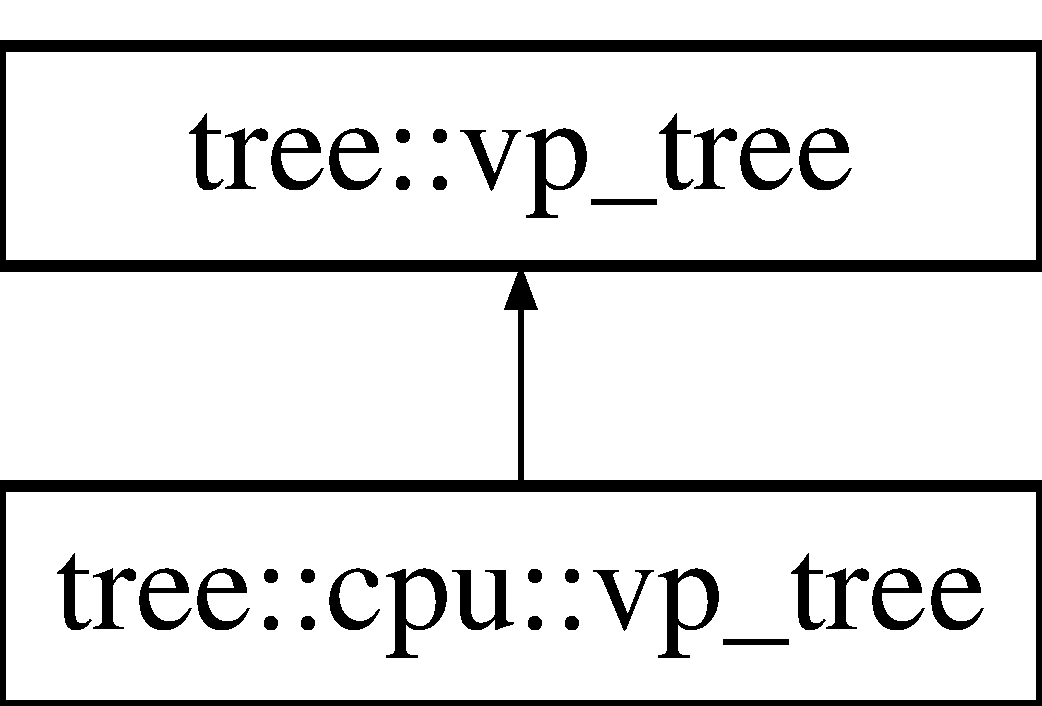
\includegraphics[height=2.000000cm]{classtree_1_1vp__tree}
\end{center}
\end{figure}
\subsection*{Public Member Functions}
\begin{DoxyCompactItemize}
\item 
\hypertarget{classtree_1_1vp__tree_a268b595d9493cf220176cda4f7dccca2}{}\hyperlink{classtree_1_1vp__tree_a268b595d9493cf220176cda4f7dccca2}{vp\+\_\+tree} ()\label{classtree_1_1vp__tree_a268b595d9493cf220176cda4f7dccca2}

\begin{DoxyCompactList}\small\item\em Constructs a new empty tree. \end{DoxyCompactList}\item 
\hypertarget{classtree_1_1vp__tree_a40549e3c3fde384b2cbdb96485301161}{}\hyperlink{classtree_1_1vp__tree_a40549e3c3fde384b2cbdb96485301161}{vp\+\_\+tree} (std\+::shared\+\_\+ptr$<$ const std\+::vector$<$ float $>$$>$ \hyperlink{classtree_1_1vp__tree_a0ac835729832f805cfde6375891f9073}{data}, int \hyperlink{classtree_1_1vp__tree_a9654dfc1b8ec7db0718f3d98a9efe5e1}{dim})\label{classtree_1_1vp__tree_a40549e3c3fde384b2cbdb96485301161}

\begin{DoxyCompactList}\small\item\em Constructs a tree with the new data and dimention. \end{DoxyCompactList}\item 
\hypertarget{classtree_1_1vp__tree_a98910f15d4574987845e36962bb64f03}{}\hyperlink{classtree_1_1vp__tree_a98910f15d4574987845e36962bb64f03}{vp\+\_\+tree} (const \hyperlink{classtree_1_1vp__tree}{vp\+\_\+tree} \&other)\label{classtree_1_1vp__tree_a98910f15d4574987845e36962bb64f03}

\begin{DoxyCompactList}\small\item\em Constructs new tree based on existing tree. \end{DoxyCompactList}\item 
\hypertarget{classtree_1_1vp__tree_ad903e1af5405b518a4775c3874dd3d37}{}void \hyperlink{classtree_1_1vp__tree_ad903e1af5405b518a4775c3874dd3d37}{fit} (std\+::shared\+\_\+ptr$<$ const std\+::vector$<$ float $>$$>$ \hyperlink{classtree_1_1vp__tree_a0ac835729832f805cfde6375891f9073}{data}, int \hyperlink{classtree_1_1vp__tree_a9654dfc1b8ec7db0718f3d98a9efe5e1}{dim})\label{classtree_1_1vp__tree_ad903e1af5405b518a4775c3874dd3d37}

\begin{DoxyCompactList}\small\item\em Constructs a new tree with the given data and dimention. \end{DoxyCompactList}\item 
\hypertarget{classtree_1_1vp__tree_a0ac835729832f805cfde6375891f9073}{}const std\+::shared\+\_\+ptr$<$ const std\+::vector$<$ float $>$ $>$ \& \hyperlink{classtree_1_1vp__tree_a0ac835729832f805cfde6375891f9073}{data} () const \label{classtree_1_1vp__tree_a0ac835729832f805cfde6375891f9073}

\begin{DoxyCompactList}\small\item\em Get data vector. \end{DoxyCompactList}\item 
\hypertarget{classtree_1_1vp__tree_a9654dfc1b8ec7db0718f3d98a9efe5e1}{}int \hyperlink{classtree_1_1vp__tree_a9654dfc1b8ec7db0718f3d98a9efe5e1}{dim} () const \label{classtree_1_1vp__tree_a9654dfc1b8ec7db0718f3d98a9efe5e1}

\begin{DoxyCompactList}\small\item\em Get dimention. \end{DoxyCompactList}\item 
std\+::shared\+\_\+ptr$<$ const std\+::vector$<$ float $>$ $>$ \& \hyperlink{classtree_1_1vp__tree_a60bbbc0833e9f9d151639f1767ef134c}{data} ()
\begin{DoxyCompactList}\small\item\em Set data vector. \end{DoxyCompactList}\item 
int \& \hyperlink{classtree_1_1vp__tree_a5863f0152d429394c404707c5f91ecc2}{dim} ()
\begin{DoxyCompactList}\small\item\em Set dimention. \end{DoxyCompactList}\end{DoxyCompactItemize}
\subsection*{Protected Attributes}
\begin{DoxyCompactItemize}
\item 
std\+::shared\+\_\+ptr$<$ const std\+::vector$<$ float $>$ $>$ \hyperlink{classtree_1_1vp__tree_ad53d34e7a1648e2b5f88ae2c66e6a44d}{\+\_\+data}
\item 
int \hyperlink{classtree_1_1vp__tree_a1c99c8567c9aa156be0f2a77487bab74}{\+\_\+dim}
\end{DoxyCompactItemize}


\subsection{Detailed Description}
Base class for creating vp-\/tree. 

\subsection{Member Function Documentation}
\hypertarget{classtree_1_1vp__tree_a60bbbc0833e9f9d151639f1767ef134c}{}\index{tree\+::vp\+\_\+tree@{tree\+::vp\+\_\+tree}!data@{data}}
\index{data@{data}!tree\+::vp\+\_\+tree@{tree\+::vp\+\_\+tree}}
\subsubsection[{data}]{\setlength{\rightskip}{0pt plus 5cm}std\+::shared\+\_\+ptr$<$ const std\+::vector$<$ float $>$ $>$ \& tree\+::vp\+\_\+tree\+::data (
\begin{DoxyParamCaption}
{}
\end{DoxyParamCaption}
)\hspace{0.3cm}{\ttfamily [inline]}}\label{classtree_1_1vp__tree_a60bbbc0833e9f9d151639f1767ef134c}


Set data vector. 

Use this function as your own responsability \hypertarget{classtree_1_1vp__tree_a5863f0152d429394c404707c5f91ecc2}{}\index{tree\+::vp\+\_\+tree@{tree\+::vp\+\_\+tree}!dim@{dim}}
\index{dim@{dim}!tree\+::vp\+\_\+tree@{tree\+::vp\+\_\+tree}}
\subsubsection[{dim}]{\setlength{\rightskip}{0pt plus 5cm}int\& tree\+::vp\+\_\+tree\+::dim (
\begin{DoxyParamCaption}
{}
\end{DoxyParamCaption}
)\hspace{0.3cm}{\ttfamily [inline]}}\label{classtree_1_1vp__tree_a5863f0152d429394c404707c5f91ecc2}


Set dimention. 

Use this function as your own responsability 

\subsection{Member Data Documentation}
\hypertarget{classtree_1_1vp__tree_ad53d34e7a1648e2b5f88ae2c66e6a44d}{}\index{tree\+::vp\+\_\+tree@{tree\+::vp\+\_\+tree}!\+\_\+data@{\+\_\+data}}
\index{\+\_\+data@{\+\_\+data}!tree\+::vp\+\_\+tree@{tree\+::vp\+\_\+tree}}
\subsubsection[{\+\_\+data}]{\setlength{\rightskip}{0pt plus 5cm}std\+::shared\+\_\+ptr$<$const std\+::vector$<$float$>$ $>$ tree\+::vp\+\_\+tree\+::\+\_\+data\hspace{0.3cm}{\ttfamily [protected]}}\label{classtree_1_1vp__tree_ad53d34e7a1648e2b5f88ae2c66e6a44d}
data \hypertarget{classtree_1_1vp__tree_a1c99c8567c9aa156be0f2a77487bab74}{}\index{tree\+::vp\+\_\+tree@{tree\+::vp\+\_\+tree}!\+\_\+dim@{\+\_\+dim}}
\index{\+\_\+dim@{\+\_\+dim}!tree\+::vp\+\_\+tree@{tree\+::vp\+\_\+tree}}
\subsubsection[{\+\_\+dim}]{\setlength{\rightskip}{0pt plus 5cm}int tree\+::vp\+\_\+tree\+::\+\_\+dim\hspace{0.3cm}{\ttfamily [protected]}}\label{classtree_1_1vp__tree_a1c99c8567c9aa156be0f2a77487bab74}
Dimention of data contained in data 

The documentation for this class was generated from the following file\+:\begin{DoxyCompactItemize}
\item 
knn/\hyperlink{vp__tree_8hpp}{vp\+\_\+tree.\+hpp}\end{DoxyCompactItemize}

\hypertarget{classtree_1_1cpu_1_1vp__tree}{}\section{tree\+:\+:cpu\+:\+:vp\+\_\+tree Class Reference}
\label{classtree_1_1cpu_1_1vp__tree}\index{tree\+::cpu\+::vp\+\_\+tree@{tree\+::cpu\+::vp\+\_\+tree}}


Base class for creating vp-\/tree.  




{\ttfamily \#include $<$vp\+\_\+tree\+\_\+cpu.\+hpp$>$}

Inheritance diagram for tree\+:\+:cpu\+:\+:vp\+\_\+tree\+:\begin{figure}[H]
\begin{center}
\leavevmode
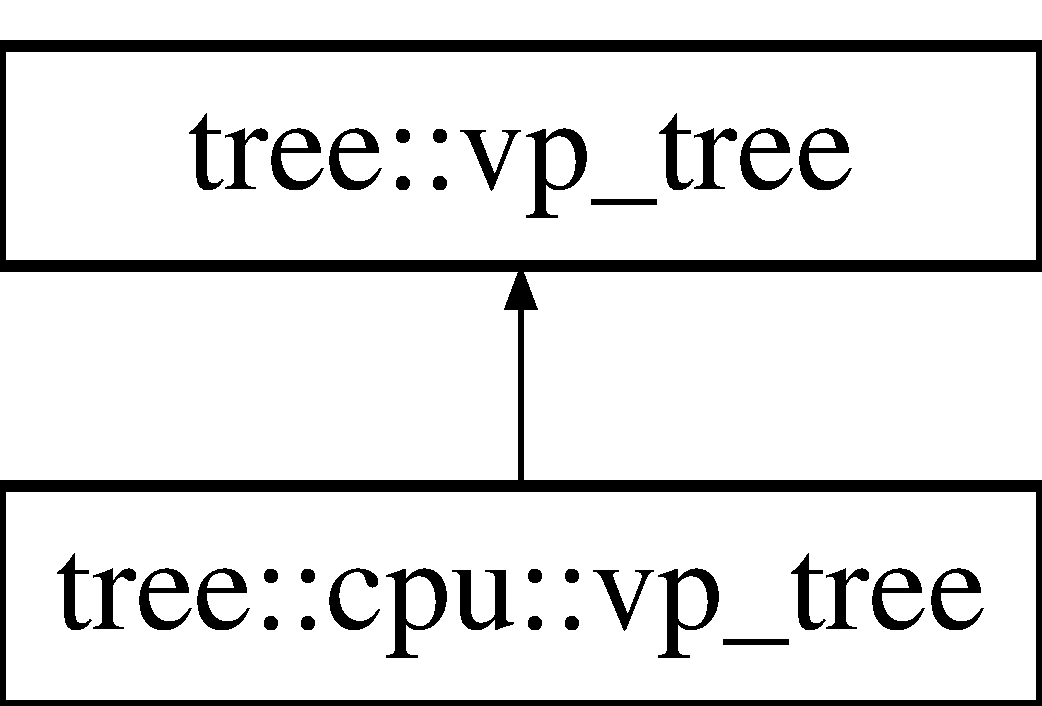
\includegraphics[height=2.000000cm]{classtree_1_1cpu_1_1vp__tree}
\end{center}
\end{figure}
\subsection*{Public Member Functions}
\begin{DoxyCompactItemize}
\item 
\hypertarget{classtree_1_1cpu_1_1vp__tree_a2ca59caf1f9c8fb271ef1a2947a69857}{}\hyperlink{classtree_1_1cpu_1_1vp__tree_a2ca59caf1f9c8fb271ef1a2947a69857}{vp\+\_\+tree} ()\label{classtree_1_1cpu_1_1vp__tree_a2ca59caf1f9c8fb271ef1a2947a69857}

\begin{DoxyCompactList}\small\item\em Constructs a new empty tree. \end{DoxyCompactList}\item 
\hyperlink{classtree_1_1cpu_1_1vp__tree_ac374600ef88cda498f56c0c74507b9da}{vp\+\_\+tree} (std\+::shared\+\_\+ptr$<$ const std\+::vector$<$ float $>$$>$ \hyperlink{classtree_1_1vp__tree_a0ac835729832f805cfde6375891f9073}{data}, int \hyperlink{classtree_1_1vp__tree_a9654dfc1b8ec7db0718f3d98a9efe5e1}{dim}, metric\+::cpu\+::metric\+\_\+f \hyperlink{classtree_1_1cpu_1_1vp__tree_a174296b009a968f5805f17ea013d06cb}{metric}=metric\+::cpu\+::euclidean)
\begin{DoxyCompactList}\small\item\em Constructs a new vp-\/tree. \end{DoxyCompactList}\item 
\hypertarget{classtree_1_1cpu_1_1vp__tree_a8119b9544df022460130563cb1a32b4b}{}\hyperlink{classtree_1_1cpu_1_1vp__tree_a8119b9544df022460130563cb1a32b4b}{vp\+\_\+tree} (const \hyperlink{classtree_1_1cpu_1_1vp__tree}{vp\+\_\+tree} \&other)\label{classtree_1_1cpu_1_1vp__tree_a8119b9544df022460130563cb1a32b4b}

\begin{DoxyCompactList}\small\item\em Copies another vp-\/tree to this object. \end{DoxyCompactList}\item 
\hypertarget{classtree_1_1cpu_1_1vp__tree_a77bbd3d462b5b464b3c775cf296c1178}{}void \hyperlink{classtree_1_1cpu_1_1vp__tree_a77bbd3d462b5b464b3c775cf296c1178}{fit} (std\+::shared\+\_\+ptr$<$ const std\+::vector$<$ float $>$$>$ \hyperlink{classtree_1_1vp__tree_a0ac835729832f805cfde6375891f9073}{data}, int \hyperlink{classtree_1_1vp__tree_a9654dfc1b8ec7db0718f3d98a9efe5e1}{dim}, metric\+::cpu\+::metric\+\_\+f \hyperlink{classtree_1_1cpu_1_1vp__tree_a174296b009a968f5805f17ea013d06cb}{metric}=metric\+::cpu\+::euclidean)\label{classtree_1_1cpu_1_1vp__tree_a77bbd3d462b5b464b3c775cf296c1178}

\begin{DoxyCompactList}\small\item\em Constructs a new tree with the given data and dimention. \end{DoxyCompactList}\item 
void \hyperlink{classtree_1_1cpu_1_1vp__tree_a5490fe2b15df7311f16893fe77f2387c}{stack\+\_\+knn} (int query, float delta, std\+::vector$<$ int $>$ \&id)
\begin{DoxyCompactList}\small\item\em Performs the knn search and returns all elements within the radius delta of the query. \end{DoxyCompactList}\item 
void \hyperlink{classtree_1_1cpu_1_1vp__tree_ab2956b54f9bfae552ee353b63b518d9f}{knn} (int query, float delta, std\+::vector$<$ int $>$ \&id)
\begin{DoxyCompactList}\small\item\em Performs the knn search and returns all elements within the radius delta of the query. \end{DoxyCompactList}\item 
void \hyperlink{classtree_1_1cpu_1_1vp__tree_a53834f76cd09227d0a094392c90f3a06}{stack\+\_\+knn} (int query, int k, std\+::vector$<$ int $>$ \&id)
\begin{DoxyCompactList}\small\item\em Performs the knn search and returns k elements closest to the query. \end{DoxyCompactList}\item 
void \hyperlink{classtree_1_1cpu_1_1vp__tree_a42daa91934422c544b2d3234d6f4b4c1}{knn} (int query, int k, std\+::vector$<$ int $>$ \&id)
\begin{DoxyCompactList}\small\item\em Performs the knn search and returns k elements closest to the query. \end{DoxyCompactList}\item 
\hypertarget{classtree_1_1cpu_1_1vp__tree_a6b4257008f872348b15ec221b6e74348}{}void \hyperlink{classtree_1_1cpu_1_1vp__tree_a6b4257008f872348b15ec221b6e74348}{brute\+\_\+knn} (int query, float delta, std\+::vector$<$ int $>$ \&id)\label{classtree_1_1cpu_1_1vp__tree_a6b4257008f872348b15ec221b6e74348}

\begin{DoxyCompactList}\small\item\em Same function as knn but using the brute force algorithm. \end{DoxyCompactList}\item 
\hypertarget{classtree_1_1cpu_1_1vp__tree_a417aef52e44c4b1f8b5d778e8e251be3}{}void \hyperlink{classtree_1_1cpu_1_1vp__tree_a417aef52e44c4b1f8b5d778e8e251be3}{brute\+\_\+knn} (int query, int k, std\+::vector$<$ int $>$ \&id)\label{classtree_1_1cpu_1_1vp__tree_a417aef52e44c4b1f8b5d778e8e251be3}

\begin{DoxyCompactList}\small\item\em Same function as knn but using the brute force algorithm. \end{DoxyCompactList}\item 
\hypertarget{classtree_1_1cpu_1_1vp__tree_a705a05444e892308fa7156968a29456d}{}int \hyperlink{classtree_1_1cpu_1_1vp__tree_a705a05444e892308fa7156968a29456d}{find} (int query) const \label{classtree_1_1cpu_1_1vp__tree_a705a05444e892308fa7156968a29456d}

\begin{DoxyCompactList}\small\item\em Finds the query in \+\_\+data vector and returns its index in the tree. \end{DoxyCompactList}\item 
\hypertarget{classtree_1_1cpu_1_1vp__tree_a30b6f89d268aae73aeb8a3125eeb631d}{}bool \hyperlink{classtree_1_1cpu_1_1vp__tree_a30b6f89d268aae73aeb8a3125eeb631d}{belongs} (int query) const \label{classtree_1_1cpu_1_1vp__tree_a30b6f89d268aae73aeb8a3125eeb631d}

\begin{DoxyCompactList}\small\item\em Brute force algorithm to check wheater a query belongs to the tree or not. \end{DoxyCompactList}\item 
\hypertarget{classtree_1_1cpu_1_1vp__tree_ad7b31aa027f85f38d293b3e0f9b37048}{}const std\+::shared\+\_\+ptr$<$ std\+::vector$<$ \hyperlink{structtree_1_1vp__node__t}{tree\+::vp\+\_\+node} $>$ $>$ \& \hyperlink{classtree_1_1cpu_1_1vp__tree_ad7b31aa027f85f38d293b3e0f9b37048}{t} () const \label{classtree_1_1cpu_1_1vp__tree_ad7b31aa027f85f38d293b3e0f9b37048}

\begin{DoxyCompactList}\small\item\em Get the tree. \end{DoxyCompactList}\item 
\hypertarget{classtree_1_1cpu_1_1vp__tree_a174296b009a968f5805f17ea013d06cb}{}const metric\+::cpu\+::metric\+\_\+f \& \hyperlink{classtree_1_1cpu_1_1vp__tree_a174296b009a968f5805f17ea013d06cb}{metric} () const \label{classtree_1_1cpu_1_1vp__tree_a174296b009a968f5805f17ea013d06cb}

\begin{DoxyCompactList}\small\item\em Gets the metric function. \end{DoxyCompactList}\item 
\hypertarget{classtree_1_1cpu_1_1vp__tree_a33f823dd101947f371a701107a8dad9d}{}metric\+::cpu\+::metric\+\_\+f \& \hyperlink{classtree_1_1cpu_1_1vp__tree_a33f823dd101947f371a701107a8dad9d}{metric} ()\label{classtree_1_1cpu_1_1vp__tree_a33f823dd101947f371a701107a8dad9d}

\begin{DoxyCompactList}\small\item\em Sets the metric function. \end{DoxyCompactList}\item 
\hypertarget{classtree_1_1cpu_1_1vp__tree_a2ce12f56df286265f5774cd7ed6591cf}{}void \hyperlink{classtree_1_1cpu_1_1vp__tree_a2ce12f56df286265f5774cd7ed6591cf}{print\+\_\+tree} ()\label{classtree_1_1cpu_1_1vp__tree_a2ce12f56df286265f5774cd7ed6591cf}

\begin{DoxyCompactList}\small\item\em prints the whole tree \end{DoxyCompactList}\item 
\hypertarget{classtree_1_1cpu_1_1vp__tree_a5d2affdc5daf2e8ad4d30fe99c7fe9ee}{}void \hyperlink{classtree_1_1cpu_1_1vp__tree_a5d2affdc5daf2e8ad4d30fe99c7fe9ee}{print\+\_\+range} (int b, int e)\label{classtree_1_1cpu_1_1vp__tree_a5d2affdc5daf2e8ad4d30fe99c7fe9ee}

\begin{DoxyCompactList}\small\item\em prints a range of the tree \end{DoxyCompactList}\item 
void \hyperlink{classtree_1_1cpu_1_1vp__tree_addb1a27773443a133c15c75309de3ee8}{check\+\_\+tree} ()
\end{DoxyCompactItemize}
\subsection*{Protected Member Functions}
\begin{DoxyCompactItemize}
\item 
\hypertarget{classtree_1_1cpu_1_1vp__tree_a1610ad0a015eb7634590fab15eddc464}{}void \hyperlink{classtree_1_1cpu_1_1vp__tree_a1610ad0a015eb7634590fab15eddc464}{dist2} (int p, std\+::vector$<$ \hyperlink{types_8hpp_a4b0dedd1120697012e61e312aa7058a8}{ifloat} $>$ \&index\+\_\+set) const \label{classtree_1_1cpu_1_1vp__tree_a1610ad0a015eb7634590fab15eddc464}

\begin{DoxyCompactList}\small\item\em Evaluates the distance between p and the set index\+\_\+set setting each float in index\+\_\+set. \end{DoxyCompactList}\item 
int \hyperlink{classtree_1_1cpu_1_1vp__tree_acba29bccad136acc95faf4be2929f207}{select\+\_\+vp} (const std\+::vector$<$ \hyperlink{types_8hpp_a4b0dedd1120697012e61e312aa7058a8}{ifloat} $>$ \&index\+\_\+set) const 
\begin{DoxyCompactList}\small\item\em Select among elements in index\+\_\+set the vantage point to split the Tree. \end{DoxyCompactList}\item 
float \hyperlink{classtree_1_1cpu_1_1vp__tree_a1959d61a75183d3f37a6923c382174bb}{split} (std\+::vector$<$ \hyperlink{types_8hpp_a4b0dedd1120697012e61e312aa7058a8}{ifloat} $>$ \&index\+\_\+set, std\+::vector$<$ \hyperlink{types_8hpp_a4b0dedd1120697012e61e312aa7058a8}{ifloat} $>$ \&lc, std\+::vector$<$ \hyperlink{types_8hpp_a4b0dedd1120697012e61e312aa7058a8}{ifloat} $>$ \&rc) const 
\begin{DoxyCompactList}\small\item\em Splits the index\+\_\+set in two sub sets such that lc and rc are aproximately the same size. \end{DoxyCompactList}\item 
\hypertarget{classtree_1_1cpu_1_1vp__tree_ae8deb69c56e005e07a663872042ac5f2}{}int \hyperlink{classtree_1_1cpu_1_1vp__tree_ae8deb69c56e005e07a663872042ac5f2}{make\+\_\+vp\+\_\+tree} (std\+::vector$<$ \hyperlink{types_8hpp_a4b0dedd1120697012e61e312aa7058a8}{ifloat} $>$ \&index\+\_\+set)\label{classtree_1_1cpu_1_1vp__tree_ae8deb69c56e005e07a663872042ac5f2}

\begin{DoxyCompactList}\small\item\em Constructs populating the \+\_\+tree vector a \hyperlink{classtree_1_1cpu_1_1vp__tree}{vp\+\_\+tree} corresponding to the data stored in the \+\_\+data vector and specified in the index\+\_\+set. \end{DoxyCompactList}\end{DoxyCompactItemize}
\subsection*{Protected Attributes}
\begin{DoxyCompactItemize}
\item 
std\+::shared\+\_\+ptr$<$ std\+::vector$<$ \hyperlink{structtree_1_1vp__node__t}{tree\+::vp\+\_\+node} $>$ $>$ \hyperlink{classtree_1_1cpu_1_1vp__tree_ada2f4290b6e25b4d4db7421b64690baa}{\+\_\+tree}
\begin{DoxyCompactList}\small\item\em Tree structure is stored here. \end{DoxyCompactList}\item 
metric\+::cpu\+::metric\+\_\+f \hyperlink{classtree_1_1cpu_1_1vp__tree_a5ad0a08e0bcc66466e24485f46671a21}{\+\_\+metric}
\begin{DoxyCompactList}\small\item\em Pointer to the metric function. \end{DoxyCompactList}\end{DoxyCompactItemize}


\subsection{Detailed Description}
Base class for creating vp-\/tree. 

\subsection{Constructor \& Destructor Documentation}
\hypertarget{classtree_1_1cpu_1_1vp__tree_ac374600ef88cda498f56c0c74507b9da}{}\index{tree\+::cpu\+::vp\+\_\+tree@{tree\+::cpu\+::vp\+\_\+tree}!vp\+\_\+tree@{vp\+\_\+tree}}
\index{vp\+\_\+tree@{vp\+\_\+tree}!tree\+::cpu\+::vp\+\_\+tree@{tree\+::cpu\+::vp\+\_\+tree}}
\subsubsection[{vp\+\_\+tree}]{\setlength{\rightskip}{0pt plus 5cm}tree\+::cpu\+::vp\+\_\+tree\+::vp\+\_\+tree (
\begin{DoxyParamCaption}
\item[{std\+::shared\+\_\+ptr$<$ const std\+::vector$<$ float $>$$>$}]{data, }
\item[{int}]{dim, }
\item[{metric\+::cpu\+::metric\+\_\+f}]{metric = {\ttfamily metric\+:\+:cpu\+:\+:euclidean}}
\end{DoxyParamCaption}
)\hspace{0.3cm}{\ttfamily [inline]}}\label{classtree_1_1cpu_1_1vp__tree_ac374600ef88cda498f56c0c74507b9da}


Constructs a new vp-\/tree. 


\begin{DoxyParams}{Parameters}
{\em data} & Data for creating vp-\/tree \\
\hline
{\em dim} & Dimention of the data \\
\hline
{\em metric} & metric function used in the vp-\/tree \\
\hline
\end{DoxyParams}


\subsection{Member Function Documentation}
\hypertarget{classtree_1_1cpu_1_1vp__tree_addb1a27773443a133c15c75309de3ee8}{}\index{tree\+::cpu\+::vp\+\_\+tree@{tree\+::cpu\+::vp\+\_\+tree}!check\+\_\+tree@{check\+\_\+tree}}
\index{check\+\_\+tree@{check\+\_\+tree}!tree\+::cpu\+::vp\+\_\+tree@{tree\+::cpu\+::vp\+\_\+tree}}
\subsubsection[{check\+\_\+tree}]{\setlength{\rightskip}{0pt plus 5cm}void tree\+::cpu\+::vp\+\_\+tree\+::check\+\_\+tree (
\begin{DoxyParamCaption}
{}
\end{DoxyParamCaption}
)\hspace{0.3cm}{\ttfamily [inline]}}\label{classtree_1_1cpu_1_1vp__tree_addb1a27773443a133c15c75309de3ee8}
checks the tree for errors \hypertarget{classtree_1_1cpu_1_1vp__tree_ab2956b54f9bfae552ee353b63b518d9f}{}\index{tree\+::cpu\+::vp\+\_\+tree@{tree\+::cpu\+::vp\+\_\+tree}!knn@{knn}}
\index{knn@{knn}!tree\+::cpu\+::vp\+\_\+tree@{tree\+::cpu\+::vp\+\_\+tree}}
\subsubsection[{knn}]{\setlength{\rightskip}{0pt plus 5cm}void tree\+::cpu\+::vp\+\_\+tree\+::knn (
\begin{DoxyParamCaption}
\item[{int}]{query, }
\item[{float}]{delta, }
\item[{std\+::vector$<$ int $>$ \&}]{id}
\end{DoxyParamCaption}
)\hspace{0.3cm}{\ttfamily [inline]}}\label{classtree_1_1cpu_1_1vp__tree_ab2956b54f9bfae552ee353b63b518d9f}


Performs the knn search and returns all elements within the radius delta of the query. 

This function does not use any stack o recursion, what makes it suitable for implementation in G\+P\+G\+P\+Us. This algorithm should be slower due to the lack of a stack and the necessity of recomputing distances 
\begin{DoxyParams}{Parameters}
{\em query} & index of query in the data \\
\hline
{\em delta} & maximum distance exclusive to search \\
\hline
{\em id} & ids of elements in data closer to query than delta \\
\hline
\end{DoxyParams}
\hypertarget{classtree_1_1cpu_1_1vp__tree_a42daa91934422c544b2d3234d6f4b4c1}{}\index{tree\+::cpu\+::vp\+\_\+tree@{tree\+::cpu\+::vp\+\_\+tree}!knn@{knn}}
\index{knn@{knn}!tree\+::cpu\+::vp\+\_\+tree@{tree\+::cpu\+::vp\+\_\+tree}}
\subsubsection[{knn}]{\setlength{\rightskip}{0pt plus 5cm}void tree\+::cpu\+::vp\+\_\+tree\+::knn (
\begin{DoxyParamCaption}
\item[{int}]{query, }
\item[{int}]{k, }
\item[{std\+::vector$<$ int $>$ \&}]{id}
\end{DoxyParamCaption}
)\hspace{0.3cm}{\ttfamily [inline]}}\label{classtree_1_1cpu_1_1vp__tree_a42daa91934422c544b2d3234d6f4b4c1}


Performs the knn search and returns k elements closest to the query. 

This function does not use any stack o recursion, what makes it suitable for implementation in G\+P\+G\+P\+Us. This algorithm should be slower due to the lack of a stack and the necessity of recomputing distances \hypertarget{classtree_1_1cpu_1_1vp__tree_acba29bccad136acc95faf4be2929f207}{}\index{tree\+::cpu\+::vp\+\_\+tree@{tree\+::cpu\+::vp\+\_\+tree}!select\+\_\+vp@{select\+\_\+vp}}
\index{select\+\_\+vp@{select\+\_\+vp}!tree\+::cpu\+::vp\+\_\+tree@{tree\+::cpu\+::vp\+\_\+tree}}
\subsubsection[{select\+\_\+vp}]{\setlength{\rightskip}{0pt plus 5cm}int tree\+::cpu\+::vp\+\_\+tree\+::select\+\_\+vp (
\begin{DoxyParamCaption}
\item[{const std\+::vector$<$ {\bf ifloat} $>$ \&}]{index\+\_\+set}
\end{DoxyParamCaption}
) const\hspace{0.3cm}{\ttfamily [inline]}, {\ttfamily [protected]}}\label{classtree_1_1cpu_1_1vp__tree_acba29bccad136acc95faf4be2929f207}


Select among elements in index\+\_\+set the vantage point to split the Tree. 

Basic implementation still. Don\textquotesingle{}t see the point for a more complicated code \hypertarget{classtree_1_1cpu_1_1vp__tree_a1959d61a75183d3f37a6923c382174bb}{}\index{tree\+::cpu\+::vp\+\_\+tree@{tree\+::cpu\+::vp\+\_\+tree}!split@{split}}
\index{split@{split}!tree\+::cpu\+::vp\+\_\+tree@{tree\+::cpu\+::vp\+\_\+tree}}
\subsubsection[{split}]{\setlength{\rightskip}{0pt plus 5cm}float tree\+::cpu\+::vp\+\_\+tree\+::split (
\begin{DoxyParamCaption}
\item[{std\+::vector$<$ {\bf ifloat} $>$ \&}]{index\+\_\+set, }
\item[{std\+::vector$<$ {\bf ifloat} $>$ \&}]{lc, }
\item[{std\+::vector$<$ {\bf ifloat} $>$ \&}]{rc}
\end{DoxyParamCaption}
) const\hspace{0.3cm}{\ttfamily [inline]}, {\ttfamily [protected]}}\label{classtree_1_1cpu_1_1vp__tree_a1959d61a75183d3f37a6923c382174bb}


Splits the index\+\_\+set in two sub sets such that lc and rc are aproximately the same size. 

\begin{DoxyReturn}{Returns}
The distance used for splitting the two subsets 
\end{DoxyReturn}
\hypertarget{classtree_1_1cpu_1_1vp__tree_a5490fe2b15df7311f16893fe77f2387c}{}\index{tree\+::cpu\+::vp\+\_\+tree@{tree\+::cpu\+::vp\+\_\+tree}!stack\+\_\+knn@{stack\+\_\+knn}}
\index{stack\+\_\+knn@{stack\+\_\+knn}!tree\+::cpu\+::vp\+\_\+tree@{tree\+::cpu\+::vp\+\_\+tree}}
\subsubsection[{stack\+\_\+knn}]{\setlength{\rightskip}{0pt plus 5cm}void tree\+::cpu\+::vp\+\_\+tree\+::stack\+\_\+knn (
\begin{DoxyParamCaption}
\item[{int}]{query, }
\item[{float}]{delta, }
\item[{std\+::vector$<$ int $>$ \&}]{id}
\end{DoxyParamCaption}
)\hspace{0.3cm}{\ttfamily [inline]}}\label{classtree_1_1cpu_1_1vp__tree_a5490fe2b15df7311f16893fe77f2387c}


Performs the knn search and returns all elements within the radius delta of the query. 

This function uses a stack for speeding up the knn search and it\textquotesingle{}s not suitable for parellization in G\+P\+G\+P\+Us 
\begin{DoxyParams}{Parameters}
{\em query} & index of query in the data \\
\hline
{\em delta} & maximum distance exclusive to search \\
\hline
{\em id} & ids of elements in data closer to query than delta \\
\hline
\end{DoxyParams}
\hypertarget{classtree_1_1cpu_1_1vp__tree_a53834f76cd09227d0a094392c90f3a06}{}\index{tree\+::cpu\+::vp\+\_\+tree@{tree\+::cpu\+::vp\+\_\+tree}!stack\+\_\+knn@{stack\+\_\+knn}}
\index{stack\+\_\+knn@{stack\+\_\+knn}!tree\+::cpu\+::vp\+\_\+tree@{tree\+::cpu\+::vp\+\_\+tree}}
\subsubsection[{stack\+\_\+knn}]{\setlength{\rightskip}{0pt plus 5cm}void tree\+::cpu\+::vp\+\_\+tree\+::stack\+\_\+knn (
\begin{DoxyParamCaption}
\item[{int}]{query, }
\item[{int}]{k, }
\item[{std\+::vector$<$ int $>$ \&}]{id}
\end{DoxyParamCaption}
)\hspace{0.3cm}{\ttfamily [inline]}}\label{classtree_1_1cpu_1_1vp__tree_a53834f76cd09227d0a094392c90f3a06}


Performs the knn search and returns k elements closest to the query. 

This function uses a stack for speeding up the knn search and it\textquotesingle{}s not suitable for parellization in G\+P\+G\+P\+Us 

\subsection{Member Data Documentation}
\hypertarget{classtree_1_1cpu_1_1vp__tree_a5ad0a08e0bcc66466e24485f46671a21}{}\index{tree\+::cpu\+::vp\+\_\+tree@{tree\+::cpu\+::vp\+\_\+tree}!\+\_\+metric@{\+\_\+metric}}
\index{\+\_\+metric@{\+\_\+metric}!tree\+::cpu\+::vp\+\_\+tree@{tree\+::cpu\+::vp\+\_\+tree}}
\subsubsection[{\+\_\+metric}]{\setlength{\rightskip}{0pt plus 5cm}metric\+::cpu\+::metric\+\_\+f tree\+::cpu\+::vp\+\_\+tree\+::\+\_\+metric\hspace{0.3cm}{\ttfamily [protected]}}\label{classtree_1_1cpu_1_1vp__tree_a5ad0a08e0bcc66466e24485f46671a21}


Pointer to the metric function. 

The metric function should return the squared distance between two elements in the data \hypertarget{classtree_1_1cpu_1_1vp__tree_ada2f4290b6e25b4d4db7421b64690baa}{}\index{tree\+::cpu\+::vp\+\_\+tree@{tree\+::cpu\+::vp\+\_\+tree}!\+\_\+tree@{\+\_\+tree}}
\index{\+\_\+tree@{\+\_\+tree}!tree\+::cpu\+::vp\+\_\+tree@{tree\+::cpu\+::vp\+\_\+tree}}
\subsubsection[{\+\_\+tree}]{\setlength{\rightskip}{0pt plus 5cm}std\+::shared\+\_\+ptr$<$std\+::vector$<${\bf tree\+::vp\+\_\+node}$>$ $>$ tree\+::cpu\+::vp\+\_\+tree\+::\+\_\+tree\hspace{0.3cm}{\ttfamily [protected]}}\label{classtree_1_1cpu_1_1vp__tree_ada2f4290b6e25b4d4db7421b64690baa}


Tree structure is stored here. 

Vector containing the vp-\/tree representation of all the data stored in \+\_\+data vector of super class 

The documentation for this class was generated from the following file\+:\begin{DoxyCompactItemize}
\item 
knn/\hyperlink{vp__tree__cpu_8hpp}{vp\+\_\+tree\+\_\+cpu.\+hpp}\end{DoxyCompactItemize}

\chapter{File Documentation}
\hypertarget{dbscan_8hpp}{}\section{clusterer/dbscan.hpp File Reference}
\label{dbscan_8hpp}\index{clusterer/dbscan.\+hpp@{clusterer/dbscan.\+hpp}}


Definition of the class base for the dbscan clusterer.  


{\ttfamily \#include \char`\"{}vp\+\_\+tree.\+hpp\char`\"{}}\\*
\subsection*{Classes}
\begin{DoxyCompactItemize}
\item 
class \hyperlink{classcluster_1_1dbscan}{cluster\+::dbscan}
\begin{DoxyCompactList}\small\item\em Base class for applying D\+B\+S\+C\+A\+N clustering algorithm to data. \end{DoxyCompactList}\end{DoxyCompactItemize}


\subsection{Detailed Description}
Definition of the class base for the dbscan clusterer. 

\begin{DoxyAuthor}{Author}
Tiago L\+O\+B\+A\+T\+O G\+I\+M\+E\+N\+E\+S (\href{mailto:tlgimenes@gmail.com}{\tt tlgimenes@gmail.\+com}) 
\end{DoxyAuthor}
\begin{DoxyDate}{Date}
2015-\/04-\/20 17\+:54
\end{DoxyDate}
This file contains the implementation of the base class for the dbscan clustering algorithm 
\hypertarget{dbscan__cpu_8hpp}{}\section{clusterer/dbscan\+\_\+cpu.hpp File Reference}
\label{dbscan__cpu_8hpp}\index{clusterer/dbscan\+\_\+cpu.\+hpp@{clusterer/dbscan\+\_\+cpu.\+hpp}}


Definition of the class specialization of dbscan for C\+P\+U.  


{\ttfamily \#include \char`\"{}dbscan.\+hpp\char`\"{}}\\*
{\ttfamily \#include \char`\"{}metrics.\+hpp\char`\"{}}\\*
{\ttfamily \#include \char`\"{}vp\+\_\+tree\+\_\+cpu.\+hpp\char`\"{}}\\*
\subsection*{Classes}
\begin{DoxyCompactItemize}
\item 
class \hyperlink{classcluster_1_1cpu_1_1dbscan}{cluster\+::cpu\+::dbscan}
\begin{DoxyCompactList}\small\item\em Class for applying D\+B\+S\+C\+A\+N clustering algorithm to data. \end{DoxyCompactList}\end{DoxyCompactItemize}


\subsection{Detailed Description}
Definition of the class specialization of dbscan for C\+P\+U. 

\begin{DoxyAuthor}{Author}
Tiago L\+O\+B\+A\+T\+O G\+I\+M\+E\+N\+E\+S (\href{mailto:tlgimenes@gmail.com}{\tt tlgimenes@gmail.\+com}) 
\end{DoxyAuthor}
\begin{DoxyDate}{Date}
2015-\/04-\/28 13\+:53
\end{DoxyDate}
This file contains the implementation of the class specialization for the dbscan clustering algorithm on C\+P\+U 
\hypertarget{metrics_8hpp}{}\section{knn/metrics.hpp File Reference}
\label{metrics_8hpp}\index{knn/metrics.\+hpp@{knn/metrics.\+hpp}}


metric definitions  


\subsection*{Typedefs}
\begin{DoxyCompactItemize}
\item 
using {\bfseries metric\+::cpu\+::metric\+\_\+f} = float($\ast$)(int, int, const std\+::vector$<$ float $>$ \&, int)
\begin{DoxyCompactList}\small\item\em Definition of the distance function used for defining the metric space. \end{DoxyCompactList}\end{DoxyCompactItemize}
\subsection*{Functions}
\begin{DoxyCompactItemize}
\item 
\hypertarget{namespacemetric_1_1cpu_ad5bbf1763fda02e7c586f15bd6796f86}{}float {\bfseries metric\+::cpu\+::euclidean} (int a, int b, const std\+::vector$<$ float $>$ \&data, int dim)\label{namespacemetric_1_1cpu_ad5bbf1763fda02e7c586f15bd6796f86}

\begin{DoxyCompactList}\small\item\em Implementation of the euclidean metric. \end{DoxyCompactList}\end{DoxyCompactItemize}


\subsection{Detailed Description}
metric definitions 

\begin{DoxyAuthor}{Author}
Tiago L\+O\+B\+A\+T\+O G\+I\+M\+E\+N\+E\+S (\href{mailto:tlgimenes@gmail.com}{\tt tlgimenes@gmail.\+com}) 
\end{DoxyAuthor}
\begin{DoxyDate}{Date}
2015-\/04-\/22 22\+:35
\end{DoxyDate}
This file contains implementation of metric functions 
\hypertarget{vp__tree_8hpp}{}\section{knn/vp\+\_\+tree.hpp File Reference}
\label{vp__tree_8hpp}\index{knn/vp\+\_\+tree.\+hpp@{knn/vp\+\_\+tree.\+hpp}}


vp\+\_\+tree base class implementation  


{\ttfamily \#include $<$vector$>$}\\*
{\ttfamily \#include $<$memory$>$}\\*
{\ttfamily \#include \char`\"{}error.\+hpp\char`\"{}}\\*
\subsection*{Classes}
\begin{DoxyCompactItemize}
\item 
struct \hyperlink{structtree_1_1vp__node__t}{tree\+::vp\+\_\+node\+\_\+t}
\begin{DoxyCompactList}\small\item\em vp-\/tree node for a linearized tree in an array \end{DoxyCompactList}\item 
class \hyperlink{classtree_1_1vp__tree}{tree\+::vp\+\_\+tree}
\begin{DoxyCompactList}\small\item\em Base class for creating vp-\/tree. \end{DoxyCompactList}\end{DoxyCompactItemize}
\subsection*{Typedefs}
\begin{DoxyCompactItemize}
\item 
\hypertarget{namespacetree_aea750986c2bbbf5a01a991f46cd911cc}{}using {\bfseries tree\+::vp\+\_\+node} = struct vp\+\_\+node\+\_\+t\label{namespacetree_aea750986c2bbbf5a01a991f46cd911cc}

\begin{DoxyCompactList}\small\item\em vp-\/tree node typedef \end{DoxyCompactList}\end{DoxyCompactItemize}
\subsection*{Functions}
\begin{DoxyCompactItemize}
\item 
\hypertarget{vp__tree_8hpp_aa90be4ebfc639dd496cc920789a34d6a}{}std\+::ostream \& \hyperlink{vp__tree_8hpp_aa90be4ebfc639dd496cc920789a34d6a}{operator$<$$<$} (std\+::ostream \&in, const \hyperlink{structtree_1_1vp__node__t}{tree\+::vp\+\_\+node} \&n)\label{vp__tree_8hpp_aa90be4ebfc639dd496cc920789a34d6a}

\begin{DoxyCompactList}\small\item\em function for printing vp\+\_\+node struct \end{DoxyCompactList}\end{DoxyCompactItemize}


\subsection{Detailed Description}
vp\+\_\+tree base class implementation 

\begin{DoxyAuthor}{Author}
Tiago L\+O\+B\+A\+T\+O G\+I\+M\+E\+N\+E\+S (\href{mailto:tlgimenes@gmail.com}{\tt tlgimenes@gmail.\+com}) 
\end{DoxyAuthor}
\begin{DoxyDate}{Date}
2015-\/04-\/20 18\+:09
\end{DoxyDate}
This file contains base class implementation of vp\+\_\+tree 
\hypertarget{vp__tree__cpu_8hpp}{}\section{knn/vp\+\_\+tree\+\_\+cpu.hpp File Reference}
\label{vp__tree__cpu_8hpp}\index{knn/vp\+\_\+tree\+\_\+cpu.\+hpp@{knn/vp\+\_\+tree\+\_\+cpu.\+hpp}}


vp\+\_\+tree cpu class especification  


{\ttfamily \#include $<$algorithm$>$}\\*
{\ttfamily \#include \char`\"{}vp\+\_\+tree.\+hpp\char`\"{}}\\*
{\ttfamily \#include \char`\"{}metrics.\+hpp\char`\"{}}\\*
{\ttfamily \#include \char`\"{}types.\+hpp\char`\"{}}\\*
{\ttfamily \#include \char`\"{}time.\+hpp\char`\"{}}\\*
\subsection*{Classes}
\begin{DoxyCompactItemize}
\item 
class \hyperlink{classtree_1_1cpu_1_1vp__tree}{tree\+::cpu\+::vp\+\_\+tree}
\begin{DoxyCompactList}\small\item\em Base class for creating vp-\/tree. \end{DoxyCompactList}\end{DoxyCompactItemize}
\subsection*{Macros}
\begin{DoxyCompactItemize}
\item 
\#define \hyperlink{vp__tree__cpu_8hpp_a002b2f4894492820fe708b1b7e7c5e70}{E\+P\+S\+I\+L\+O\+N}~1e-\/6
\begin{DoxyCompactList}\small\item\em Float comparision threshold. \end{DoxyCompactList}\item 
\#define \hyperlink{vp__tree__cpu_8hpp_a62e90d5c1b5aad7ab60823163cc2f2d7}{L\+E\+A\+F}~-\/1
\item 
\#define \hyperlink{vp__tree__cpu_8hpp_a77988da40e9a35da51ea0e8943ebbd4a}{R\+O\+O\+T}~-\/2
\item 
\#define \hyperlink{vp__tree__cpu_8hpp_abde25a67f4046530ae1c572cefeb5869}{U\+N\+D\+E\+F}~-\/3
\end{DoxyCompactItemize}


\subsection{Detailed Description}
vp\+\_\+tree cpu class especification 

\begin{DoxyAuthor}{Author}
Tiago L\+O\+B\+A\+T\+O G\+I\+M\+E\+N\+E\+S (\href{mailto:tlgimenes@gmail.com}{\tt tlgimenes@gmail.\+com}) 
\end{DoxyAuthor}
\begin{DoxyDate}{Date}
2015-\/04-\/20 21\+:58
\end{DoxyDate}
This file contains the cpu specialization of vp\+\_\+tree class 

\subsection{Macro Definition Documentation}
\hypertarget{vp__tree__cpu_8hpp_a002b2f4894492820fe708b1b7e7c5e70}{}\index{vp\+\_\+tree\+\_\+cpu.\+hpp@{vp\+\_\+tree\+\_\+cpu.\+hpp}!E\+P\+S\+I\+L\+O\+N@{E\+P\+S\+I\+L\+O\+N}}
\index{E\+P\+S\+I\+L\+O\+N@{E\+P\+S\+I\+L\+O\+N}!vp\+\_\+tree\+\_\+cpu.\+hpp@{vp\+\_\+tree\+\_\+cpu.\+hpp}}
\subsubsection[{E\+P\+S\+I\+L\+O\+N}]{\setlength{\rightskip}{0pt plus 5cm}\#define E\+P\+S\+I\+L\+O\+N~1e-\/6}\label{vp__tree__cpu_8hpp_a002b2f4894492820fe708b1b7e7c5e70}


Float comparision threshold. 

If the modulus of the difference between two floats is smaller than this value the float values are considered to be equal \hypertarget{vp__tree__cpu_8hpp_a62e90d5c1b5aad7ab60823163cc2f2d7}{}\index{vp\+\_\+tree\+\_\+cpu.\+hpp@{vp\+\_\+tree\+\_\+cpu.\+hpp}!L\+E\+A\+F@{L\+E\+A\+F}}
\index{L\+E\+A\+F@{L\+E\+A\+F}!vp\+\_\+tree\+\_\+cpu.\+hpp@{vp\+\_\+tree\+\_\+cpu.\+hpp}}
\subsubsection[{L\+E\+A\+F}]{\setlength{\rightskip}{0pt plus 5cm}\#define L\+E\+A\+F~-\/1}\label{vp__tree__cpu_8hpp_a62e90d5c1b5aad7ab60823163cc2f2d7}
Leaf descriptor \hypertarget{vp__tree__cpu_8hpp_a77988da40e9a35da51ea0e8943ebbd4a}{}\index{vp\+\_\+tree\+\_\+cpu.\+hpp@{vp\+\_\+tree\+\_\+cpu.\+hpp}!R\+O\+O\+T@{R\+O\+O\+T}}
\index{R\+O\+O\+T@{R\+O\+O\+T}!vp\+\_\+tree\+\_\+cpu.\+hpp@{vp\+\_\+tree\+\_\+cpu.\+hpp}}
\subsubsection[{R\+O\+O\+T}]{\setlength{\rightskip}{0pt plus 5cm}\#define R\+O\+O\+T~-\/2}\label{vp__tree__cpu_8hpp_a77988da40e9a35da51ea0e8943ebbd4a}
Root descriptor \hypertarget{vp__tree__cpu_8hpp_abde25a67f4046530ae1c572cefeb5869}{}\index{vp\+\_\+tree\+\_\+cpu.\+hpp@{vp\+\_\+tree\+\_\+cpu.\+hpp}!U\+N\+D\+E\+F@{U\+N\+D\+E\+F}}
\index{U\+N\+D\+E\+F@{U\+N\+D\+E\+F}!vp\+\_\+tree\+\_\+cpu.\+hpp@{vp\+\_\+tree\+\_\+cpu.\+hpp}}
\subsubsection[{U\+N\+D\+E\+F}]{\setlength{\rightskip}{0pt plus 5cm}\#define U\+N\+D\+E\+F~-\/3}\label{vp__tree__cpu_8hpp_abde25a67f4046530ae1c572cefeb5869}
Undefined node descriptor 
\hypertarget{parser_8hpp}{}\section{parser/parser.hpp File Reference}
\label{parser_8hpp}\index{parser/parser.\+hpp@{parser/parser.\+hpp}}


C\+L\+I parser.  


{\ttfamily \#include $<$string$>$}\\*
{\ttfamily \#include $<$cstring$>$}\\*
{\ttfamily \#include $<$utility$>$}\\*
{\ttfamily \#include $<$map$>$}\\*
{\ttfamily \#include \char`\"{}error.\+hpp\char`\"{}}\\*
\subsection*{Classes}
\begin{DoxyCompactItemize}
\item 
class \hyperlink{classconsole_1_1parser}{console\+::parser}
\begin{DoxyCompactList}\small\item\em Class for parsing the Command Line Interface. \end{DoxyCompactList}\end{DoxyCompactItemize}
\subsection*{Macros}
\begin{DoxyCompactItemize}
\item 
\hypertarget{parser_8hpp_a2b44836e554e7e07d65ece4ae251c06c}{}\#define \hyperlink{parser_8hpp_a2b44836e554e7e07d65ece4ae251c06c}{D\+E\+F\+A\+U\+L\+T\+\_\+\+S\+T\+R\+I\+N\+G}~\char`\"{}0\char`\"{}\label{parser_8hpp_a2b44836e554e7e07d65ece4ae251c06c}

\begin{DoxyCompactList}\small\item\em Default string to be returned in case of failure. \end{DoxyCompactList}\end{DoxyCompactItemize}


\subsection{Detailed Description}
C\+L\+I parser. 

\begin{DoxyAuthor}{Author}
Tiago L\+O\+B\+A\+T\+O G\+I\+M\+E\+N\+E\+S (\href{mailto:tlgimenes@gmail.com}{\tt tlgimenes@gmail.\+com}) 
\end{DoxyAuthor}
\begin{DoxyDate}{Date}
2015-\/03-\/30 15\+:05
\end{DoxyDate}
This file contains implementation of a simple C\+L\+I parser 
\hypertarget{color_8hpp}{}\section{utils/color.hpp File Reference}
\label{color_8hpp}\index{utils/color.\+hpp@{utils/color.\+hpp}}


color C\+L\+I modifier  


{\ttfamily \#include $<$ostream$>$}\\*
\subsection*{Classes}
\begin{DoxyCompactItemize}
\item 
class \hyperlink{classconsole_1_1modifier}{console\+::modifier}
\end{DoxyCompactItemize}
\subsection*{Enumerations}
\begin{DoxyCompactItemize}
\item 
\hypertarget{namespaceconsole_af545da495907ceb52e8e85ca1a357698}{}enum {\bfseries ccode} \{ \\*
{\bfseries F\+G\+\_\+\+R\+E\+D} = 31, 
{\bfseries F\+G\+\_\+\+G\+R\+E\+E\+N} = 32, 
{\bfseries F\+G\+\_\+\+Y\+E\+L\+L\+O\+W} = 33, 
{\bfseries F\+G\+\_\+\+B\+L\+U\+E} = 34, 
\\*
{\bfseries F\+G\+\_\+\+M\+A\+G\+E\+N\+T\+A} = 35, 
{\bfseries F\+G\+\_\+\+C\+Y\+A\+N} = 36, 
{\bfseries F\+G\+\_\+\+L\+\_\+\+G\+R\+A\+Y} = 37, 
{\bfseries F\+G\+\_\+\+D\+\_\+\+G\+R\+A\+Y} = 90, 
\\*
{\bfseries F\+G\+\_\+\+D\+E\+F\+A\+U\+L\+T} = 39, 
{\bfseries B\+G\+\_\+\+R\+E\+D} = 41, 
{\bfseries B\+G\+\_\+\+G\+R\+E\+E\+N} = 42, 
{\bfseries B\+G\+\_\+\+Y\+E\+L\+L\+O\+W} = 43, 
\\*
{\bfseries B\+G\+\_\+\+B\+L\+U\+E} = 44, 
{\bfseries B\+G\+\_\+\+M\+A\+G\+E\+N\+T\+A} = 45, 
{\bfseries B\+G\+\_\+\+C\+Y\+A\+N} = 46, 
{\bfseries B\+G\+\_\+\+L\+\_\+\+G\+R\+A\+Y} = 47, 
\\*
{\bfseries B\+G\+\_\+\+D\+\_\+\+G\+R\+A\+Y} = 100, 
{\bfseries B\+G\+\_\+\+D\+E\+F\+A\+U\+L\+T} = 49, 
{\bfseries S\+E\+T\+\_\+\+B\+O\+L\+D} = 1, 
{\bfseries S\+E\+T\+\_\+\+D\+I\+M} = 2, 
\\*
{\bfseries R\+E\+S\+E\+T\+\_\+\+B\+O\+L\+D} = 21, 
{\bfseries R\+E\+S\+E\+T\+\_\+\+D\+I\+M} = 22, 
{\bfseries D\+E\+F\+A\+U\+L\+T} = 0
 \}\label{namespaceconsole_af545da495907ceb52e8e85ca1a357698}

\begin{DoxyCompactList}\small\item\em Color code for the modifier. \end{DoxyCompactList}\end{DoxyCompactItemize}


\subsection{Detailed Description}
color C\+L\+I modifier 

\begin{DoxyAuthor}{Author}
Tiago L\+O\+B\+A\+T\+O G\+I\+M\+E\+N\+E\+S (\href{mailto:tlgimenes@gmail.com}{\tt tlgimenes@gmail.\+com}) 
\end{DoxyAuthor}
\begin{DoxyDate}{Date}
2015-\/04-\/27 13\+:43
\end{DoxyDate}
This file contains a class implementation that allows to change colors in the terminal. If the terminal does not support colors, some strange character chains will be printed 
\hypertarget{error_8hpp}{}\section{utils/error.hpp File Reference}
\label{error_8hpp}\index{utils/error.\+hpp@{utils/error.\+hpp}}


error repporting interface  


{\ttfamily \#include $<$string$>$}\\*
{\ttfamily \#include $<$chrono$>$}\\*
{\ttfamily \#include $<$iostream$>$}\\*
{\ttfamily \#include \char`\"{}color.\+hpp\char`\"{}}\\*
\subsection*{Macros}
\begin{DoxyCompactItemize}
\item 
\hypertarget{error_8hpp_a75bd11cb87e859cbefc91ad4ca92c993}{}\#define \hyperlink{error_8hpp_a75bd11cb87e859cbefc91ad4ca92c993}{D\+B\+G\+\_\+\+M\+E\+S\+S\+A\+G\+E}(str)~\+\_\+\+\_\+message(str, console\+::\+F\+G\+\_\+\+D\+\_\+\+G\+R\+A\+Y)\label{error_8hpp_a75bd11cb87e859cbefc91ad4ca92c993}

\begin{DoxyCompactList}\small\item\em Message to be displayed in debug only mode. \end{DoxyCompactList}\item 
\#define \hyperlink{error_8hpp_a480a5c17233ad51db62c0b98c4126fae}{F\+A\+T\+A\+L\+\_\+\+E\+R\+R\+O\+R}(str)~\+\_\+\+\_\+error(str, \+\_\+\+\_\+\+F\+I\+L\+E\+\_\+\+\_\+, \+\_\+\+\_\+\+L\+I\+N\+E\+\_\+\+\_\+)
\begin{DoxyCompactList}\small\item\em Fatal errors. \end{DoxyCompactList}\item 
\#define \hyperlink{error_8hpp_a1df547c3e0d42a7bde3b7f962172ffc3}{W\+A\+R\+N\+I\+N\+G\+\_\+\+E\+R\+R\+O\+R}(str)~\+\_\+\+\_\+warning(str, \+\_\+\+\_\+\+F\+I\+L\+E\+\_\+\+\_\+, \+\_\+\+\_\+\+L\+I\+N\+E\+\_\+\+\_\+)
\begin{DoxyCompactList}\small\item\em Warning. \end{DoxyCompactList}\item 
\hypertarget{error_8hpp_aa1f978ce2192133033cb44c2f545eea3}{}\#define \hyperlink{error_8hpp_aa1f978ce2192133033cb44c2f545eea3}{A\+S\+S\+E\+R\+T\+\_\+\+F\+A\+T\+A\+L\+\_\+\+E\+R\+R\+O\+R}(boolean,  str)~(void)((boolean) $\vert$$\vert$ (\+\_\+\+\_\+error(str, \+\_\+\+\_\+\+F\+I\+L\+E\+\_\+\+\_\+, \+\_\+\+\_\+\+L\+I\+N\+E\+\_\+\+\_\+),0))\label{error_8hpp_aa1f978ce2192133033cb44c2f545eea3}

\begin{DoxyCompactList}\small\item\em Asserts with fatal error message. \end{DoxyCompactList}\item 
\hypertarget{error_8hpp_aee4df526c9d8a9912494b9b05f640b7d}{}\#define \hyperlink{error_8hpp_aee4df526c9d8a9912494b9b05f640b7d}{A\+S\+S\+E\+R\+T\+\_\+\+W\+A\+R\+N\+I\+N\+G\+\_\+\+E\+R\+R\+O\+R}(boolean,  str)~(void)((boolean) $\vert$$\vert$ (\+\_\+\+\_\+warning(str, \+\_\+\+\_\+\+F\+I\+L\+E\+\_\+\+\_\+, \+\_\+\+\_\+\+L\+I\+N\+E\+\_\+\+\_\+),0))\label{error_8hpp_aee4df526c9d8a9912494b9b05f640b7d}

\begin{DoxyCompactList}\small\item\em Asserts with warning message. \end{DoxyCompactList}\item 
\#define \hyperlink{error_8hpp_adc5c9f0985775005b835304b1722af95}{C\+U\+D\+A\+\_\+\+S\+A\+F\+E}(code)~\hyperlink{error_8hpp_aa1f978ce2192133033cb44c2f545eea3}{A\+S\+S\+E\+R\+T\+\_\+\+F\+A\+T\+A\+L\+\_\+\+E\+R\+R\+O\+R}(code == cuda\+Success, cuda\+Get\+Error\+String(cuda\+Get\+Last\+Error()))
\begin{DoxyCompactList}\small\item\em This macro searches for errors in cuda functions execution. \end{DoxyCompactList}\end{DoxyCompactItemize}


\subsection{Detailed Description}
error repporting interface 

\begin{DoxyAuthor}{Author}
Tiago L\+O\+B\+A\+T\+O G\+I\+M\+E\+N\+E\+S (\href{mailto:tlgimenes@gmail.com}{\tt tlgimenes@gmail.\+com}) 
\end{DoxyAuthor}
\begin{DoxyDate}{Date}
2015-\/02-\/02 11\+:13
\end{DoxyDate}
This file contains the implementation of a simple error repporting interface 

\subsection{Macro Definition Documentation}
\hypertarget{error_8hpp_adc5c9f0985775005b835304b1722af95}{}\index{error.\+hpp@{error.\+hpp}!C\+U\+D\+A\+\_\+\+S\+A\+F\+E@{C\+U\+D\+A\+\_\+\+S\+A\+F\+E}}
\index{C\+U\+D\+A\+\_\+\+S\+A\+F\+E@{C\+U\+D\+A\+\_\+\+S\+A\+F\+E}!error.\+hpp@{error.\+hpp}}
\subsubsection[{C\+U\+D\+A\+\_\+\+S\+A\+F\+E}]{\setlength{\rightskip}{0pt plus 5cm}\#define C\+U\+D\+A\+\_\+\+S\+A\+F\+E(
\begin{DoxyParamCaption}
\item[{}]{code}
\end{DoxyParamCaption}
)~{\bf A\+S\+S\+E\+R\+T\+\_\+\+F\+A\+T\+A\+L\+\_\+\+E\+R\+R\+O\+R}(code == cuda\+Success, cuda\+Get\+Error\+String(cuda\+Get\+Last\+Error()))}\label{error_8hpp_adc5c9f0985775005b835304b1722af95}


This macro searches for errors in cuda functions execution. 

One should use always this macro in each cuda function call \hypertarget{error_8hpp_a480a5c17233ad51db62c0b98c4126fae}{}\index{error.\+hpp@{error.\+hpp}!F\+A\+T\+A\+L\+\_\+\+E\+R\+R\+O\+R@{F\+A\+T\+A\+L\+\_\+\+E\+R\+R\+O\+R}}
\index{F\+A\+T\+A\+L\+\_\+\+E\+R\+R\+O\+R@{F\+A\+T\+A\+L\+\_\+\+E\+R\+R\+O\+R}!error.\+hpp@{error.\+hpp}}
\subsubsection[{F\+A\+T\+A\+L\+\_\+\+E\+R\+R\+O\+R}]{\setlength{\rightskip}{0pt plus 5cm}\#define F\+A\+T\+A\+L\+\_\+\+E\+R\+R\+O\+R(
\begin{DoxyParamCaption}
\item[{}]{str}
\end{DoxyParamCaption}
)~\+\_\+\+\_\+error(str, \+\_\+\+\_\+\+F\+I\+L\+E\+\_\+\+\_\+, \+\_\+\+\_\+\+L\+I\+N\+E\+\_\+\+\_\+)}\label{error_8hpp_a480a5c17233ad51db62c0b98c4126fae}


Fatal errors. 

This macro writes the error message in str and exits \hypertarget{error_8hpp_a1df547c3e0d42a7bde3b7f962172ffc3}{}\index{error.\+hpp@{error.\+hpp}!W\+A\+R\+N\+I\+N\+G\+\_\+\+E\+R\+R\+O\+R@{W\+A\+R\+N\+I\+N\+G\+\_\+\+E\+R\+R\+O\+R}}
\index{W\+A\+R\+N\+I\+N\+G\+\_\+\+E\+R\+R\+O\+R@{W\+A\+R\+N\+I\+N\+G\+\_\+\+E\+R\+R\+O\+R}!error.\+hpp@{error.\+hpp}}
\subsubsection[{W\+A\+R\+N\+I\+N\+G\+\_\+\+E\+R\+R\+O\+R}]{\setlength{\rightskip}{0pt plus 5cm}\#define W\+A\+R\+N\+I\+N\+G\+\_\+\+E\+R\+R\+O\+R(
\begin{DoxyParamCaption}
\item[{}]{str}
\end{DoxyParamCaption}
)~\+\_\+\+\_\+warning(str, \+\_\+\+\_\+\+F\+I\+L\+E\+\_\+\+\_\+, \+\_\+\+\_\+\+L\+I\+N\+E\+\_\+\+\_\+)}\label{error_8hpp_a1df547c3e0d42a7bde3b7f962172ffc3}


Warning. 

This macro writes the warning message in str and continues 
\hypertarget{reader__xtc_8hpp}{}\section{utils/reader\+\_\+xtc.hpp File Reference}
\label{reader__xtc_8hpp}\index{utils/reader\+\_\+xtc.\+hpp@{utils/reader\+\_\+xtc.\+hpp}}


.xtc file reader  


{\ttfamily \#include $<$vector$>$}\\*
{\ttfamily \#include $<$string$>$}\\*
{\ttfamily \#include $<$sstream$>$}\\*
{\ttfamily \#include $<$fstream$>$}\\*
{\ttfamily \#include $<$boost/filesystem.\+hpp$>$}\\*
{\ttfamily \#include \char`\"{}error.\+hpp\char`\"{}}\\*
{\ttfamily \#include \char`\"{}xdrfile/xdrfile.\+h\char`\"{}}\\*
{\ttfamily \#include \char`\"{}xdrfile/xdrfile\+\_\+xtc.\+h\char`\"{}}\\*
\subsection*{Classes}
\begin{DoxyCompactItemize}
\item 
class \hyperlink{classreader__xtc}{reader\+\_\+xtc}
\begin{DoxyCompactList}\small\item\em Class for reading trajlist and .xtc files. \end{DoxyCompactList}\end{DoxyCompactItemize}
\subsection*{Macros}
\begin{DoxyCompactItemize}
\item 
\hypertarget{reader__xtc_8hpp_a9958e549a943ec37c7fbb33685befb02}{}\#define \hyperlink{reader__xtc_8hpp_a9958e549a943ec37c7fbb33685befb02}{M\+A\+X\+\_\+\+F\+I\+L\+E\+\_\+\+N\+A\+M\+E\+\_\+\+L\+E\+N\+G\+T\+H}~128\label{reader__xtc_8hpp_a9958e549a943ec37c7fbb33685befb02}

\begin{DoxyCompactList}\small\item\em Maximun file name lenght. \end{DoxyCompactList}\end{DoxyCompactItemize}


\subsection{Detailed Description}
.xtc file reader 

\begin{DoxyAuthor}{Author}
Tiago L\+O\+B\+A\+T\+O G\+I\+M\+E\+N\+E\+S (\href{mailto:tlgimenes@gmail.com}{\tt tlgimenes@gmail.\+com}) 
\end{DoxyAuthor}
\begin{DoxyDate}{Date}
2015-\/03-\/30 18\+:49
\end{DoxyDate}
This file contains the implementation of a class for reading .xtc files with a trajectory list 
\hypertarget{time_8hpp}{}\section{utils/time.hpp File Reference}
\label{time_8hpp}\index{utils/time.\+hpp@{utils/time.\+hpp}}


functions and tools for mesuring the execution time of a given code  


{\ttfamily \#include $<$string$>$}\\*
{\ttfamily \#include $<$iostream$>$}\\*
{\ttfamily \#include $<$vector$>$}\\*
{\ttfamily \#include \char`\"{}color.\+hpp\char`\"{}}\\*
{\ttfamily \#include \char`\"{}error.\+hpp\char`\"{}}\\*
\subsection*{Macros}
\begin{DoxyCompactItemize}
\item 
\#define \hyperlink{time_8hpp_ad94f94f8eb7d963f13889b4f0de2689b}{C\+P\+P99}~199711\+L
\item 
\hypertarget{time_8hpp_a5d486dc52b56255d7473266d578b04f2}{}\#define \hyperlink{time_8hpp_a5d486dc52b56255d7473266d578b04f2}{T\+I\+M\+E\+\_\+\+B\+E\+T\+W\+E\+E\+N}(code)~\hyperlink{error_8hpp_a1df547c3e0d42a7bde3b7f962172ffc3}{W\+A\+R\+N\+I\+N\+G\+\_\+\+E\+R\+R\+O\+R}(\char`\"{}T\+I\+M\+E\+\_\+\+B\+E\+T\+W\+E\+E\+N needs at least C++11 compliant compiler\char`\"{})\label{time_8hpp_a5d486dc52b56255d7473266d578b04f2}

\begin{DoxyCompactList}\small\item\em Measures the execution time between the code given. \end{DoxyCompactList}\end{DoxyCompactItemize}


\subsection{Detailed Description}
functions and tools for mesuring the execution time of a given code 

\begin{DoxyAuthor}{Author}
Tiago L\+O\+B\+A\+T\+O G\+I\+M\+E\+N\+E\+S (\href{mailto:tlgimenes@gmail.com}{\tt tlgimenes@gmail.\+com}) 
\end{DoxyAuthor}
\begin{DoxyDate}{Date}
2015-\/04-\/21 18\+:36
\end{DoxyDate}
This file contains the implementation of functions for mesuring the execution time between code. It\textquotesingle{}s necessary to have C++11 support 

\subsection{Macro Definition Documentation}
\hypertarget{time_8hpp_ad94f94f8eb7d963f13889b4f0de2689b}{}\index{time.\+hpp@{time.\+hpp}!C\+P\+P99@{C\+P\+P99}}
\index{C\+P\+P99@{C\+P\+P99}!time.\+hpp@{time.\+hpp}}
\subsubsection[{C\+P\+P99}]{\setlength{\rightskip}{0pt plus 5cm}\#define C\+P\+P99~199711\+L}\label{time_8hpp_ad94f94f8eb7d963f13889b4f0de2689b}
C++99 version number 
\hypertarget{types_8hpp}{}\section{utils/types.hpp File Reference}
\label{types_8hpp}\index{utils/types.\+hpp@{utils/types.\+hpp}}


Simple type definitions.  


{\ttfamily \#include $<$cstdarg$>$}\\*
{\ttfamily \#include \char`\"{}error.\+hpp\char`\"{}}\\*
\subsection*{Classes}
\begin{DoxyCompactItemize}
\item 
class \hyperlink{classprimitive}{primitive$<$ T, N $>$}
\begin{DoxyCompactList}\small\item\em Implementation of general N-\/dimentional type. \end{DoxyCompactList}\item 
class \hyperlink{classkey__value}{key\+\_\+value$<$ K, V $>$}
\begin{DoxyCompactList}\small\item\em Key-\/\+Value class implementation. \end{DoxyCompactList}\end{DoxyCompactItemize}
\subsection*{Typedefs}
\begin{DoxyCompactItemize}
\item 
{\footnotesize template$<$int N$>$ }\\using \hyperlink{types_8hpp_acb451bae75ebf80f56e8ce537c9fc5ac}{floatn} = \hyperlink{classprimitive}{primitive}$<$ float, N $>$
\item 
{\footnotesize template$<$int N$>$ }\\using \hyperlink{types_8hpp_ae0cdc1093ce32adcc52a246cea2064c6}{intn} = \hyperlink{classprimitive}{primitive}$<$ int, N $>$
\item 
using \hyperlink{types_8hpp_a9d85ec097fc4152573afe09e6817b150}{float4} = \hyperlink{types_8hpp_acb451bae75ebf80f56e8ce537c9fc5ac}{floatn}$<$ 4 $>$
\item 
using \hyperlink{types_8hpp_a4b0dedd1120697012e61e312aa7058a8}{ifloat} = \hyperlink{classkey__value}{key\+\_\+value}$<$ int, float $>$
\end{DoxyCompactItemize}


\subsection{Detailed Description}
Simple type definitions. 

\begin{DoxyAuthor}{Author}
Tiago L\+O\+B\+A\+T\+O G\+I\+M\+E\+N\+E\+S (\href{mailto:tlgimenes@gmail.com}{\tt tlgimenes@gmail.\+com}) 
\end{DoxyAuthor}
\begin{DoxyDate}{Date}
2015-\/04-\/21 15\+:10
\end{DoxyDate}
This file contains the implementation and definition of simple types imeplemented on C\+U\+D\+A and Open\+C\+L 

\subsection{Typedef Documentation}
\hypertarget{types_8hpp_a9d85ec097fc4152573afe09e6817b150}{}\index{types.\+hpp@{types.\+hpp}!float4@{float4}}
\index{float4@{float4}!types.\+hpp@{types.\+hpp}}
\subsubsection[{float4}]{\setlength{\rightskip}{0pt plus 5cm}using {\bf float4} =  {\bf floatn}$<$4$>$}\label{types_8hpp_a9d85ec097fc4152573afe09e6817b150}
4-\/\+Dimentional float definition \hypertarget{types_8hpp_acb451bae75ebf80f56e8ce537c9fc5ac}{}\index{types.\+hpp@{types.\+hpp}!floatn@{floatn}}
\index{floatn@{floatn}!types.\+hpp@{types.\+hpp}}
\subsubsection[{floatn}]{\setlength{\rightskip}{0pt plus 5cm}template$<$int N$>$ using {\bf floatn} =  {\bf primitive}$<$float, N$>$}\label{types_8hpp_acb451bae75ebf80f56e8ce537c9fc5ac}
N-\/\+Dimentional float definition \hypertarget{types_8hpp_a4b0dedd1120697012e61e312aa7058a8}{}\index{types.\+hpp@{types.\+hpp}!ifloat@{ifloat}}
\index{ifloat@{ifloat}!types.\+hpp@{types.\+hpp}}
\subsubsection[{ifloat}]{\setlength{\rightskip}{0pt plus 5cm}using {\bf ifloat} =  {\bf key\+\_\+value}$<$int, float$>$}\label{types_8hpp_a4b0dedd1120697012e61e312aa7058a8}
Indexed float (ifloat) definition \hypertarget{types_8hpp_ae0cdc1093ce32adcc52a246cea2064c6}{}\index{types.\+hpp@{types.\+hpp}!intn@{intn}}
\index{intn@{intn}!types.\+hpp@{types.\+hpp}}
\subsubsection[{intn}]{\setlength{\rightskip}{0pt plus 5cm}template$<$int N$>$ using {\bf intn} =  {\bf primitive}$<$int, N$>$}\label{types_8hpp_ae0cdc1093ce32adcc52a246cea2064c6}
N-\/\+Dimentional int definition 
%--- End generated contents ---

% Index
\backmatter
\newpage
\phantomsection
\clearemptydoublepage
\addcontentsline{toc}{chapter}{Index}
\printindex

\end{document}
